% !TEX root = main_ilyi.tex

% for pdfLaTeX
\pdfoutput=1

\documentclass[11pt]{article}

% Change "review" to "final" to generate the final (sometimes called camera-ready) version.
% Change to "preprint" to generate a non-anonymous version with page numbers.
\usepackage{lib}

% Standard package includes
\usepackage{times}
\usepackage{latexsym}

% For proper rendering and hyphenation of words containing Latin characters (including in bib files)
\usepackage[T1]{fontenc}

% This assumes your files are encoded as UTF8
\usepackage[utf8]{inputenc}

\usepackage{microtype}

\usepackage{inconsolata}

\usepackage{graphicx}
\usepackage{amsmath}
\usepackage{multirow}
\usepackage{booktabs}
\usepackage{amssymb}
\usepackage{hyperref}


% If the title and author information does not fit in the area allocated, uncomment the following
%
%\setlength\titlebox{<dim>}
%
% and set <dim> to something 5cm or larger.

\title{Multimodal Information Extraction of Supermarket Leaflets}

\author{Ilyesse Hettenbach\textsuperscript{}, Gabriel Schurr\textsuperscript{} \\
HKA, Karlsruhe, Germany \\
\texttt{\{heil1012, scga1011\}@h-ka.de} \\
\href{https://github.com/ilyii/leaflets}{https://github.com/ilyii/leaflets}
}


\begin{document}
\maketitle
\begin{abstract}
TODO
\end{abstract}

\section{Introduction}

\subsection{Motivation}
If one thinks of a paper-heavy country, Germany is likely to come to mind. The country's affinity for printed materials is deeply ingrained in its culture, with activities such as browsing through supermarket leaflets serving as a familiar ritual for many individuals. These leaflets have long been an essential medium for consumers to plan their purchases, discover special offers, and compare prices. The tactile nature of printed leaflets, the excitement of spotting discounts, and the satisfaction of making a well-informed shopping decision contribute to their enduring appeal.
However, the rapid advancement of digital technology is transforming consumer behavior. While some individuals still find browsing through physical leaflets a nostalgic and even relaxing experience, younger generations are increasingly turning to digital alternatives for their shopping needs. The modern shopper expects convenience, efficiency, and instant access to information, yet the digital transformation of supermarket leaflets lags significantly behind other aspects of e-commerce and retail technology.

Despite the existence of applications that compile digital versions of these leaflets, their usability and overall quality remain suboptimal. Many digital leaflets are plain documents, failing to leverage the full potential of interactivity, searchability, and intelligent recommendation systems. There is a pressing need for sophisticated digital solutions that not only present supermarket deals but also enable consumers to interact with them in a meaningful way. 

Possibly, one can imagine a seamless digital platform where users can search for specific items across multiple supermarket chains, apply dietary filters to instantly highlight suitable products, or receive personalized recommendations based on past preferences. A tool that allows consumers to create a dynamic shopping list, track price trends over time, and receive real-time updates on the best deals would revolutionize the way people approach grocery shopping. Yet, these features remain largely absent from existing digital leaflet solutions. Furthermore, while price comparison websites and applications have become commonplace for electronics, fashion, and travel, the grocery sector remains an overlooked frontier. Consumers are often left navigating multiple supermarket websites or manually cross-referencing prices to find the best deals—a tedious and inefficient process. A comprehensive digital ecosystem that integrates grocery price comparisons, personalized discounts, and AI-driven shopping assistants could bridge this gap and act as a workaround, offering an enhanced, data-driven shopping experience tailored to individual needs.

The future of supermarket deal discovery should not be a static PDF or an unorganized collection of scanned pages—it should be a dynamic, interactive, and intelligent experience that aligns with the evolving digital landscape.

\subsection{Problem Statement}
The primary objective of this research is to develop an intelligent system for extracting, structuring, and utilizing information from supermarket leaflets in a digital format. Given a set of supermarket leaflets \(\mathcal{L} = \{L_1, L_2, ..., L_n\}\), each containing a collection of product deals with specific attributes such as product name, brand, price, discount, product image and other product specifications, the goal is to extract and normalize these attributes to enable efficient querying and comparison across multiple supermarket chains.

Each leaflet \( L_i \) consists of a set of $m$ product entries \( P_i = \{p_1, p_2, ..., p_m\} \), where each product \( p_j \) is associated with a set of varying attributes: 

\begin{equation}
    p_j = \{a_1, a_2, ..., a_k\},   
\end{equation}
where each attribute \( a_k \) represents a specific entity. Common attributes include:
\begin{itemize}
    \item Product Name
    \item Brand
    \item Original Price
    \item Deal Price
    \item Unit (e.g., weight, volume)
    \item Product Image
\end{itemize}
among others. Each attribute may or may not be present in a given product entry, and the format and layout of these attributes can vary significantly across different leaflets.

To enable advanced applications such as the abovementioned, one has to tackle different challenges, such as:
% Nummerierung der Challenges
\begin{enumerate}
    \item Detecting and separating deals $p$ from the leaflet $L$.
    \item Extracting structured information from the detected deals.
    \item Normalizing the extracted information to ensure consistency and comparability.
    \item Validating the extracted information to ensure accuracy.
\end{enumerate}

Therefore, a function $$f: \mathcal{L} \to \mathcal{D}$$ has to be designed, where $\mathcal{D}$ represents the structured information extracted from the leaflets. The function $f$ should minimize the extraction error $E$.


\subsection{Contributions}  
This work presents a comprehensive approach to digitalizing and structuring supermarket leaflet information by leveraging advanced computer vision, OCR, and language models. The key contributions of this research are as follows:  

% 1. **Development of a Detection and Extraction Pipeline for Supermarket Leaflets**  
\indent{\textbf{Development of a Detection and Extraction Pipeline for Supermarket Leaflets.}} We propose a modular and efficient pipeline for detecting, extracting, and structuring information from supermarket leaflets. This pipeline integrates OCR-based text extraction, image processing, and layout understanding to accurately associate textual and visual elements such as product names, prices, descriptions, and images. Additionally, we incorporate normalization techniques to standardize extracted data across different retailers and formats.  

% 2. **Design of an Interactive Application for Deal Browsing and Price Comparison**  
\indent{\textbf{Design of an Interactive Application for Deal Browsing and Price Comparison.}} To facilitate practical use, we wrap the extracted data into a user-friendly application that enables consumers to browse, filter, and compare deals across multiple supermarket chains. This application includes basic functionalities to search, track and compare deals across different supermarket chains.

% 3. **Comprehensive Evaluation of Information Extraction Models**  
\indent{\textbf{Comprehensive Evaluation of Information Extraction Models.}} We systematically evaluate multiple state-of-the-art models for supermarket leaflet information extraction, including hybrid OCR+LLM approaches, end-to-end Vision-Language Models (VLMs), and Large Vision-Language Models (LVLMs). Our evaluation covers accuracy metrics such as per-entity correctness, Levenshtein distance, and robustness across different supermarket layouts and textual formats. This analysis provides insights into the trade-offs between computational efficiency and extraction performance.

% 4. **Training of Custom Deal Detection and Information Extraction Models**  
\indent{\textbf{Training of Custom Deal Detection and Information Extraction Models.}} To further improve extraction performance, we develop and fine-tune specialized models for deal detection and information extraction. This includes training custom object detection models to identify product regions within leaflets, as well as domain-specific sequence-to-sequence models for structured text extraction. These models are designed to enhance recognition accuracy, particularly for complex layouts and noisy scan conditions.

% 5. **Creation of a Benchmark Dataset: Leaflet-IE**  
\indent{\textbf{Creation of a Benchmark Dataset: Leaflet-IE.}} We introduce **Leaflet-IE**, a novel dataset curated for supermarket leaflet information extraction. The dataset consists of annotated images spanning multiple supermarket chains, with labeled entities including product names, prices, discounts, brands, and categories. This dataset serves as a benchmark for future research in structured information extraction from promotional materials and contributes to advancing OCR and multimodal learning for real-world retail applications.
    


\section{Related Works}
\indent{\textbf{Deal Detection}.}
\indent{\textbf{Optical Character Recognition}.}
OCR-Model-Driven methods use OCR tools to acquire text
and bounding box information. Subsequently, they rely
on the models to integrate text, layout, and visual data.

\indent{\textbf{Information Extraction}.}

\section{Nature of Supermarket Leaflet Data}
Supermarket leaflets constitute a complex and heterogeneous data source, characterized by multimodal content that combines structured and unstructured information. This data presents unique challenges for computational processing due to its inherent ambiguities, multi-instance object representations, and spatial dependencies. The reader is encouraged to simultaneously inspect the visual representation of these challenges in \figref{fig:leaflet_data} while proceeding with the discussion.

One of the primary challenges lies in the ambiguity of price recognition, where a single product may be associated with multiple price points, such as discounted prices, bulk purchase offers, or tiered pricing structures. This ambiguity is further exacerbated by errors in punctuation extraction, particularly in recognizing decimal places, which often arise from font-specific artifacts or noisy backgrounds. Resolving such issues requires advanced plausibility checks, contextual reasoning, and robust numerical interpretation mechanisms to ensure accurate data extraction. Additionally, the non-strict one-to-one mapping between textual and visual elements introduces further complexity. For instance, a single product image may represent multiple items, or textual descriptions may not align precisely with their corresponding visual representations. This misalignment necessitates sophisticated multimodal fusion techniques to bridge the gap between visual and textual data, ensuring accurate association and interpretation of product information.

The inconsistent layouts of supermarket leaflets further complicate data extraction. Promotional deals and product information are often placed in varying positions across different leaflets, making it difficult to design a universal extraction method that generalizes across diverse formats. Text elements frequently overlap with product images or other textual information, leading to misidentification or incorrect parsing of data. These challenges are compounded by the variability in fonts, sizes, and weights used within a single leaflet, which complicates the differentiation between product names, prices, and promotional tags. The presence of multilingual content and special characters adds another layer of complexity, as leaflets may contain text in multiple languages or stylized symbols that require optical character recognition (OCR) and natural language processing (NLP) models capable of handling diverse linguistic structures and alphabet systems.

Promotion labels and discount representations introduce additional challenges due to their non-standard or highly stylized text formats. Identifying the exact nature of promotions, such as "Buy 1, get 1 free" or "20\% off," requires precise extraction and interpretation, particularly when the text is embedded in noisy backgrounds or overlaps with other elements. Furthermore, the temporal context of deals and promotions adds a critical dimension to the extraction process. Some offers may only be valid for specific periods, and extracting and associating the correct date ranges with these offers can be challenging, especially when the information is not explicitly stated or is presented in ambiguous formats.

Therefore, the nature of supermarket leaflet data necessitates an advanced toolkit of visual and textual processing, analysis, extraction and generation techniques to effectively interpret and utilize the information contained within these documents. The subsequent sections will delve into the methodologies and models used to address these challenges and extract structured information from supermarket leaflets.

\section{Deal Detection}
    \subsection{Datasets}
    \subsection{Model}
    \subsection{Experiments}

\section{Information Extraction of Supermarket Deals}
Subsequently to the detection and separation of supermarket deals, the overarching goal of using these in applications requires the extraction of the various useful information from these deals. 
The task of extracting meaningful and structured information from supermarket deal images is a complex and multi-faceted problem, requiring the integration of various modalities, overcoming challenges posed by noisy data, and leveraging deep learning techniques. This section provides a detailed exploration of the underlying challenges, methodologies, and the theoretical and practical framework needed to perform such extraction.

\subsection{Challenges in Information Extraction for Supermarket Deals}

Supermarket deal extraction involves a series of challenges that require careful attention and sophisticated methods to resolve. These challenges include the diversity of layout and format in the images, the multimodal nature of the data, the frequent occurrence of Optical Character Recognition (OCR) errors, and the specific linguistic and cultural issues posed by the German language.

% \subsubsection{High Variety in Layouts and Visual Elements}
\indent{\textbf{High Variety in Layouts and Visual Elements.}}
Supermarket deals exhibit considerable variability in layout, color schemes, font choices, and text sizes, which hinders automatic detection and extraction. Deals are often printed with superscripted decimals or without clear separation between integer and fractional components of the price (e.g., "2.29" might appear as "229"). This phenomenon exacerbates OCR difficulties. Additionally, original prices may be struck through, while deal prices are sometimes printed in drastically different fonts than those the OCR model was trained on. Furthermore, overlapping elements—such as product images or additional textual information—often interfere with text extraction and localization. These diverse visual elements require robust and flexible models capable of accommodating such variability.

% \subsubsection{Multimodal Information}
\indent{\textbf{Multimodal Information.}}
Supermarket deal images consist of both visual (e.g., product images) and textual (e.g., brand names, prices, and product descriptions) modalities, each contributing different types of information. While text provides rich information about the product’s identity, pricing, and units, the image serves as a supplementary modality that aids in product identification, brand recognition, and other visual cues. Multimodal fusion, where information from both text and image domains is integrated, is a key challenge, and existing models must effectively leverage both sources to provide high-quality extraction.

\indent{\textbf{Conversion Errors and Linguistic Challenges.}}
OCR systems frequently introduce errors, particularly when dealing with non-standard fonts, noisy backgrounds, or small text. This is particularly problematic when extracting numerical data such as prices. Common errors include misinterpretation of decimals and digits (e.g., "229" instead of "2.29") and missing characters. To address this, OCR post-processing steps, such as error correction using context-based reasoning or dedicated error models, are required. Additionally, the presence of proper nouns—particularly brand names—adds complexity, as these entities may not appear in typical language models, making their extraction difficult. Furthermore, the German language presents its own set of challenges, including compound words, specific punctuation conventions, and diverse word forms, all of which must be accounted for in any robust extraction model.

\indent{\textbf{Ambiguities.}}
The presence of overlapping elements—whether textual or graphical—can lead to a degradation in the extraction accuracy. This challenge is compounded when the overlap involves essential information, such as when the original price is partially obscured by a product image or strike-through marks. Furthermore, ambiguity in labeling and the context in which different pieces of information appear in the deal image can create difficulties in associating text with the correct object (e.g., associating a price with a product rather than the surrounding descriptive text).

\subsection{Formal Approach}
Formally, the task of information extraction from a deal image can be defined as the identification of specific entities, including the product name, brand, original price, deal price, and unit. We define the following set of output labels:
\begin{equation}
\mathcal{Y} = \{y_{i}\}_{i=1}^{n},
\end{equation}
where \(y_{i}\) represents the $i$-th entity in the deal image. In the following, the entities are defined as:
\begin{itemize}
    \item \code{\(y_{\text{product\_name}}\)}: The name of the product.
    \item \code{\(y_{\text{brand}}\)}: The brand of the product.
    \item \code{\(y_{\text{original\_price}}\)}: The original price of the product.
    \item \code{\(y_{\text{deal\_price}}\)}: The deal price of the product.
    \item \code{\(y_{\text{unit}}\)}: The unit of the product (e.g., weight, volume).
\end{itemize}

To extract these entities, one aims to learn a function \(f(\cdot)\) that maps an input image \(I\) to the desired outputs:
\begin{equation}
    f: I \to \mathcal{Y},
\end{equation}
where \( I \) is the deal image, and \( \mathcal{Y} \) represents the extracted entities.

The choice of the function \( f(\cdot) \) is an architectural decision that depends on the specific requirements of the task, the nature of the data, the available resources, and the desired performance metrics. 

\subsection{Architectural Approaches to Information Extraction}
Among the various existing architectural approaches to information extraction, several methodologies have been developed to address the inherent complexities in supermarket deal images. These methods can be categorized into classical approaches, multi-stage traditional models, hybrid OCR-LLM systems, and end-to-end deep learning frameworks. Each paradigm offers distinct advantages, and their applicability depends on computational resources, dataset characteristics, and performance requirements.

\subsubsection{Traditional and Hybrid Approaches for Supermarket Leaflet Information Extraction}  
Information extraction from supermarket leaflets has traditionally been approached through a pipeline of sequential sub-tasks, each addressed by specialized systems. These methods, while extensively studied and methodologically diverse, are typically divided into three main stages: text detection, text recognition, and key-value pair extraction. Although effective in certain scenarios, these approaches suffer from inherent limitations, including computational overhead, error propagation, and suboptimal performance on edge cases. Recent advancements in large language models (LLMs) have led to the development of hybrid OCR-LLM architectures, which combine the precision of optical character recognition (OCR) with the contextual reasoning capabilities of LLMs. Below, we formalize these approaches and discuss their strengths and limitations.

Traditional architectures decompose the problem into independent sub-tasks, each handled by specialized models. While this modularity allows for targeted optimization, it introduces complexity and inefficiencies due to the lack of end-to-end training and error propagation across stages.

The first stage, \emph{text detection}, involves identifying regions in the image \( I \in \mathbb{R}^{H \times W \times 3} \) that contain textual information. This is typically achieved using rule-based systems or neural networks designed for small object detection. The output is a set of \( M \) bounding boxes \( \{b_i\}_{i=1}^{M} \), where each \( b_i = (x_{\text{min}}, y_{\text{min}}, x_{\text{max}}, y_{\text{max}}}) \) defines the coordinates of a text region. Modern approaches often employ convolutional neural networks (CNNs) or transformer-based architectures to improve robustness to varying fonts, orientations, and overlapping text.

Each detected bounding box \( b_i \) is cropped and processed by a \emph{text recognition} model to convert the visual representation into a textual one. This task is challenging due to decoding errors caused by noisy backgrounds, stylized fonts, and ambiguous characters. Commonly used models include convolutional recurrent neural networks (CRNNs) \cite{shi2016crnn} and transformer-based recognizers. Given the set of bounding boxes \( \{b_i\}_{i=1}^{M} \), the goal is to predict the corresponding textual entities \( \{t_i\}_{i=1}^{M} \):  
\[
\{t_i\}_{i=1}^{M} = \arg\max_{\{t_i\}_{i=1}^{M}} P(\{t_i\}_{i=1}^{M} | \{b_i\}_{i=1}^{M}).
\]  
The text recognition stage is often optimized using connectionist temporal classification (CTC) loss or sequence-to-sequence objectives, depending on the model architecture.

The final stage structures the extracted text into meaningful entities, such as product names, prices, and promotional tags. Named entity recognition (NER) models or graph neural networks (GNNs) are commonly used to learn associations between textual elements. The objective is to maximize the alignment score \( \Psi(v_i, v_j) \) between related entities:  
\[
\mathcal{A}^* = \arg\max_{\mathcal{A} \subseteq E} \sum_{(i,j) \in \mathcal{A}} \Psi(v_i, v_j),
\]  
where \( E \) represents textual adjacency relationships. This stage is critical for resolving ambiguities, such as associating prices with the correct products.

While traditional pipelines are widely used, they suffer from several limitations. The need for multiple independently trained models increases computational overhead and complicates system management. Additionally, the lack of end-to-end training often leads to suboptimal performance, particularly on edge cases or unseen data, as errors propagate through the pipeline.

The rise of large language models (LLMs) has enabled the development of hybrid OCR-LLM architectures, which combine the strengths of OCR tools with the linguistic and reasoning capabilities of LLMs. These approaches retain the traditional OCR pipeline for converting visual text into machine-readable form but leverage LLMs to enhance robustness through contextual reasoning and structured output generation.

In a hybrid OCR-LLM system, the OCR stage processes the input image \( I \) to produce a set of unstructured text fragments \( T = \{t_i\}_{i=1}^{M} \) with associated spatial coordinates. These fragments are serialized into a prompt \( \mathbf{P} \) and fed into a pretrained LLM \( F_\theta \), which performs contextual parsing and generates structured output \( \hat{y} \):  
\[
\hat{y} = F_\theta (T).
\]  
The LLM leverages its pretrained knowledge to resolve ambiguities, infer relationships between text fragments, and generate outputs in a structured format (e.g., JSON). For example, it can distinguish between bulk pricing (e.g., "2 for \$4") and unit pricing (e.g., "\$2 each") through arithmetic reasoning embedded in its attention mechanisms.
 
Hybrid OCR-LLM models offer several advantages over traditional pipelines. By integrating contextual reasoning, they reduce error propagation and improve robustness to noisy or ambiguous inputs. Additionally, the use of pretrained LLMs eliminates the need for task-specific training, simplifying system development. However, these models still rely on the accuracy of the OCR stage, and misrecognitions (e.g., "O" vs. "0") can propagate to the LLM. Furthermore, the computational cost of LLM inference can be prohibitive for large-scale applications.

\subsubsection{End-to-End Models}
End-to-End (E2E) approaches eliminate pipeline fragmentation by learning a unified mapping $F: I \to \mathcal{D}$.

\indent{\textbf{Vision-Encoder-Decoder Models.}} These models represent a paradigm shift in document understanding by unifying text detection, recognition, and semantic parsing into a single end-to-end trainable framework. Among these, the Donut architecture \cite{kim2022donut} has emerged as a state-of-the-art model for tasks such as information extraction from supermarket leaflets. Donut eliminates the need for intermediate OCR steps by directly mapping input images to structured outputs, leveraging a transformer-based encoder-decoder architecture. Below, we formalize the Donut model, its mathematical foundations, and its application to supermarket leaflet data.

Donut consists of two primary components: a vision encoder and a text decoder, both built on transformer layers. Given an input image \( I \in \mathbb{R}^{H \times W \times 3} \), the model generates a structured output \( \mathbf{Y} \) in an autoregressive manner. The encoder extracts high-level visual features, while the decoder translates these features into a sequence of tokens representing the desired output format.

The \emph{vision encoder} processes the input image \( I \) into a sequence of visual embeddings \( \mathbf{Z} = \{z_i\}_{i=1}^{L} \), where \( L \) is the sequence length. This is achieved using a Swin Transformer \cite{liu2021swin}, which partitions the image into non-overlapping patches and applies hierarchical self-attention to capture both local and global context. Let \( \mathbf{X} \in \mathbb{R}^{N \times (P^2 \cdot C)} \) denote the patch embeddings, where \( N \) is the number of patches, \( P \) is the patch size, and \( C \) is the number of input channels. The Swin Transformer computes multi-head self-attention (MSA) and feed-forward network (FFN) operations as follows:  
\[
\mathbf{X}' = \text{MSA}(\text{LayerNorm}(\mathbf{X})) + \mathbf{X},  
\]  
\[
\mathbf{Z} = \text{FFN}(\text{LayerNorm}(\mathbf{X}')) + \mathbf{X}',
\]  
where LayerNorm denotes layer normalization. The output \( \mathbf{Z} \) serves as the visual representation for the decoder.

The \emph{text decoder} is a transformer-based autoregressive model that generates the output sequence \( \mathbf{Y} = (y_1, y_2, \dots, y_T) \) conditioned on the visual embeddings \( \mathbf{Z} \). At each time step \( t \), the decoder predicts the next token \( y_t \) based on the previously generated tokens \( y_{<t} \) and the encoder output \( \mathbf{Z} \). The decoder computes self-attention over the output sequence and cross-attention over the visual embeddings:  
\[
\mathbf{Q} = \mathbf{W}_Q \mathbf{H}_{t-1}, \quad \mathbf{K} = \mathbf{W}_K \mathbf{Z}, \quad \mathbf{V} = \mathbf{W}_V \mathbf{Z},
\]  
\[
\text{Cross-Attention}(\mathbf{Q}, \mathbf{K}, \mathbf{V}) = \text{softmax}\left(\frac{\mathbf{Q} \mathbf{K}^\top}{\sqrt{d_k}}\right) \mathbf{V},
\]  
where \( \mathbf{H}_{t-1} \) is the hidden state at step \( t-1 \), and \( \mathbf{W}_Q, \mathbf{W}_K, \mathbf{W}_V \) are learnable projection matrices. The final token probabilities are computed as:  
\[
P(y_t | y_{<t}, \mathbf{Z}) = \text{softmax}(\mathbf{W}_o \mathbf{H}_t),
\]  
where \( \mathbf{W}_o \) is an output projection matrix. The model is trained end-to-end using a cross-entropy loss:  
\[
\mathcal{L} = -\sum_{t=1}^T \log P(y_t^* | y_{<t}, \mathbf{Z}),
\]  
where \( y_t^* \) is the ground-truth token at step \( t \).

Donut is particularly well-suited for supermarket leaflet data due to its ability to handle multimodal inputs and generate structured outputs without intermediate OCR steps. The model can directly process leaflet images and produce JSON representations of product information. By eliminating the need for OCR, it avoids error propagation and simplifies the pipeline. Its end-to-end trainability ensures optimal performance, and its ability to generate structured outputs reduces the need for post-processing. However, Donut requires large-scale pretraining on diverse document datasets, which can be computationally expensive. Additionally, its performance on low-resolution or highly noisy images may be suboptimal, as the vision encoder relies on high-quality visual features.

\indent\textbf{Large Vision-Language Models.} Large Vision-Language Models (LVLMs) represent the latest advancement in multimodal learning, combining the strengths of LLMs and vision encoders to achieve state-of-the-art performance on a wide range of tasks. These models, such as CLIP \cite{radford2021clip} and ALIGN \cite{li2022align}, leverage large-scale pretraining on diverse multimodal datasets to learn robust representations of visual and textual information. Below, we formalize the ALIGN model and discuss its application to supermarket leaflet data.

\section{Large Vision-Language Models for Supermarket Leaflet Understanding}  
Large Vision-Language Models (LVLMs) represent a transformative advancement in multimodal artificial intelligence, unifying visual perception and linguistic reasoning within a single cohesive framework. These models, such as LLaVA \cite{liu2023llava} and GPT-4V \cite{openai2023gpt4}, eliminate the traditional separation between vision and language processing by jointly encoding images and text into a shared latent space. For supermarket leaflet analysis, LVLMs enable end-to-end extraction of structured information directly from raw images, bypassing explicit OCR stages while leveraging contextual synergies between visual and textual data. We formalize the architectural principles, mathematical foundations, and application-specific adaptations of LVLMs below.

---

### **Architecture and Mathematical Formulation**  
LVLMs integrate a vision encoder, a language model, and cross-modal fusion mechanisms into a unified architecture. Given an input leaflet image \( I \in \mathbb{R}^{H \times W \times 3} \), the model generates structured textual output \( \mathbf{Y} \) through joint reasoning over visual and linguistic features.

#### **Vision Encoder**  
The vision encoder processes \( I \) into a sequence of patch embeddings \( \mathbf{Z} \in \mathbb{R}^{L \times d_v} \), where \( L \) is the number of patches and \( d_v \) is the embedding dimension. A Vision Transformer (ViT) \cite{dosovitskiy2020vit} is commonly employed, partitioning \( I \) into \( N \) non-overlapping patches \( \{\mathbf{p}_i\}_{i=1}^N \), linearly projecting each patch, and applying transformer layers with self-attention:  
\[
\mathbf{z}_i = \text{MSA}(\mathbf{p}_i) + \mathbf{p}_i, \quad \mathbf{Z} = [\mathbf{z}_1; \mathbf{z}_2; \dots; \mathbf{z}_N],
\]  
where MSA denotes multi-head self-attention. For supermarket leaflets, the encoder captures spatial relationships critical for disambiguating overlapping text and product layouts.

#### **Cross-Modal Fusion**  
Visual embeddings \( \mathbf{Z} \) are aligned with textual representations through a cross-modal projector, which maps \( \mathbf{Z} \) into the language model's embedding space. Let \( \mathbf{W}_p \in \mathbb{R}^{d_v \times d_t} \) denote a learnable projection matrix, where \( d_t \) is the language model's hidden dimension. The projected visual tokens \( \mathbf{V} \) are computed as:  
\[
\mathbf{V} = \mathbf{Z} \mathbf{W}_p.
\]  
These tokens are concatenated with text token embeddings \( \mathbf{E}_{\text{text}} \in \mathbb{R}^{T \times d_t} \) to form a unified input sequence:  
\[
\mathbf{H}_{\text{in}} = [\mathbf{V}; \mathbf{E}_{\text{text}}].
\]

#### **Language Model Decoding**  
The language model (e.g., LLaMA \cite{touvron2023llama}) processes \( \mathbf{H}_{\text{in}} \) autoregressively to generate structured output \( \mathbf{Y} = (y_1, \dots, y_T) \). At each step \( t \), cross-attention layers attend to visual tokens \( \mathbf{V} \) while self-attention layers model dependencies within the output sequence:  
\[
\mathbf{Q}_t = \mathbf{W}_Q \mathbf{h}_{t-1}, \quad \mathbf{K}_v = \mathbf{W}_K \mathbf{V}, \quad \mathbf{V}_v = \mathbf{W}_V \mathbf{V},
\]  
\[
\mathbf{h}_t' = \text{softmax}\left(\frac{\mathbf{Q}_t \mathbf{K}_v^\top}{\sqrt{d_t}}\right) \mathbf{V}_v + \mathbf{h}_{t-1},
\]  
\[
P(y_t | y_{<t}, \mathbf{Z}) = \text{softmax}(\mathbf{W}_o \mathbf{h}_t'),
\]  
where \( \mathbf{W}_Q, \mathbf{W}_K, \mathbf{W}_V, \mathbf{W}_o \) are learnable parameters. The model is trained end-to-end using a cross-entropy loss:  
\[
\mathcal{L} = -\sum_{t=1}^T \log P(y_t^* | y_{<t}, \mathbf{Z}),
\]  
where \( y_t^* \) is the ground-truth token.

---

### **Application to Supermarket Leaflets**  
LVLMs excel at extracting structured product information (e.g., prices, promotions) by jointly reasoning over visual and textual cues. For instance, given a leaflet image with the text "\$2.99" adjacent to an apple image, the model infers the association through cross-attention, generating output:  
\[
\{\text{product: "Apples", price: 2.99, promotion: "Weekly Special"}\}.
\]  
Key advantages include:  
1. **Ambiguity Resolution**: Differentiates prices from non-price numerals (e.g., "2 lbs") via contextual alignment of text and images.  
2. **Layout Robustness**: Leverages spatial attention to associate scattered text fragments (e.g., disclaimers linked to products).  
3. **Multilingual Support**: Inherits multilingual capabilities from pretrained language models, handling leaflets with mixed languages.

---

### **Advantages and Limitations**  
LVLMs eliminate error-prone OCR pipelines and enable zero-shot generalization through their pretrained knowledge. Their unified architecture simplifies deployment and reduces computational overhead compared to hybrid OCR-LLM systems. However, limitations persist:  
- **Training Complexity**: Requires large-scale multimodal datasets (e.g., leaflet images paired with JSON outputs) for fine-tuning.  
- **Hallucination Risks**: May generate plausible but incorrect details if visual grounding is weak (e.g., inventing prices for occluded text).  
- **Resource Intensity**: High memory and compute demands during inference, limiting real-time applications.  

---

### **Conclusion**  
Large Vision-Language Models redefine supermarket leaflet information extraction by unifying visual and linguistic reasoning into an end-to-end framework. Their ability to directly map raw images to structured outputs, bypassing intermediate OCR stages, positions them as a promising solution for complex retail document understanding. Future work should focus on enhancing visual grounding, optimizing inference efficiency, and expanding multilingual support to address current limitations.

\subsection{Dataset Creation}
Since the availability of German supermarket leaflet data is literally not findable, a custom dataset was created by manually annotating a collection of supermarket deal images. The dataset includes images from the most common supermarket chains, each with unique layout, fonts, and colors to, in general, ensure the highest diversity and robustness possible. Each image is annotated with a corresponding label file that includes the desired entities as well as the image identificator. The dataset is split into a training (~ 80\%) and a validation set (~ 20\%) for each model to be trained and evaluated on. Table \tabref{tab:ie_dataset} provides an overview of the dataset with the sample size for each entity and \figref{fig:ie_dataset_samples} shows some sample images with their annotations.

\begin{table}[ht]
\centering
\caption{Leaflet-IE Dataset}
\label{tab:ie_dataset}
\begin{tabular}{lc}
\toprule
Entity           & Sample Size \\
\midrule
\code{image\_id}        & 372  \\
\code{brand}            & 357  \\
\code{product\_name}    & 370  \\
\code{original\_price}  & 286  \\
\code{deal\_price}      & 372  \\
\code{weight}           & 369  \\
\bottomrule
\end{tabular}
\end{table}

Even though the Leaflet-IE dataset is relatively small, the reader will be able to see that the dataset is sufficient to evaluate the performance of different IE appraoches as well as to train an competitive end-to-end model. However, as the reader may notice, the dataset is solely focused on single product deals at this point and explicitly does not include 

\begin{figure*}[ht]
\centering
\fbox{\parbox[c][3cm][c]{5cm}{\centering Figure Placeholder: Sample Annotation}}
\caption{Sample images with annotations from the custom dataset.}
\label{fig:ie_dataset_samples}
\end{figure*}

\section{Experiments}

The primary objective of these experiments is to identify the most effective approach for extracting structured information from supermarket leaflets. The evaluation considers general performance trends and use cases to determine candidate methodologies, including Hybrid OCR + LLM, end-to-end Vision-Encoder-Decoder models, and LVLMs.
The order of the experiments is as follows:
- Plain Deal OCR Performance
- OCR + LLM Performance
- Donut Fine-Tuning Performance
- MAIN: Comparison of Hybrid OCR+LLM, Donut, and LVLM


\subsection{Implementation Details}
The experiments were conducted on two distinct computational workstations - station 1 equipped with an NVIDIA RTX 4080 GPU and station 2 with an NVIDIA GTX 1080 GPU. Therefore, the experiments could be conducted in parallel, ensuring efficient model training and evaluation.

The software stack includegraphics Python with PyTorch as the primary deep learning framework, HuggingFace Transformers for leveraging pre-trained models, and OpenCV for image preprocessing and data augmentation.
 PyTorch, HuggingFace Transformers, and various other libraries for data pre-and post-processing, visualization, data management and monitoring \footnote{The codebase is available at \href{https://github.com/ilyii/leaflets}{https://github.com/ilyii/leaflets}}.


% SUB-STUDIES
\subsection{Plain Deal OCR Performance}
The aim of this experiment is to evaluate the performance of various OCR models in extracting text from supermarket leaflets. The evaluation focuses on the accuracies of the extracted entities from \tabref{tab:ie_dataset} and the impact of different normalization levels on the recognition performance. The results provide insights into the robustness and accuracy of different OCR models in handling the complexities of supermarket leaflet data.

The most commonly used OCR models include:
\begin{itemize}
    \item Tesseract,
    \item EasyOCR,
    \item PaddleOCR,
    \item DocTR.
\end{itemize}
These models have been trained on a variety of datasets and are known for their robustness and accuracy in text extraction. Since it is likely that none of the OCR models have seen this data before, all 372 samples of the Leaflet-IE dataset were used for evaluation. While OCR alone is not capable of generating key-value mappings, the evaluation used a different set of metrics:

\begin{itemize}
    \item \textbf{Accuracy}: Measures whether the expected value is present in the OCR output.
    \item \textbf{N-gram Accuracy}: Determines if an n-gram substring of the expected value exists in the OCR output, computed for \(n \in \left[\frac{|v|}{2}, |v| - 1\right]\), where \(|v|\) represents the string length of the ground truth entity value.
\end{itemize}

Given that language-specific OCR errors are common, the evaluation was conducted at different levels of normalization to improve comparability. The text normalization included the following layers:
\begin{itemize}
    \item \textbf{Level 1:} Text stripping and string conversion.
    \item \textbf{Level 2:} Lowercasing and basic replacements.
    \item \textbf{Level 3:} Use-case specific replacements.
    \item \textbf{Level 4:} Punctuation and whitespace removal.
\end{itemize}
Each level includes the normalization steps of the previous levels. Therefore, the normalization procedure can be thought of as a gradual alignment of the OCR output to the ground truth to investigate the OCR model's robustness to different normalization levels.


\indent{\textbf{Results}.} Figure \ref{fig:eval_ocr_accuracies} presents a comparative analysis of various OCR models and normalization levels based on per-entity accuracy. The results highlight several key trends regarding the recognition performance of different entities.

\begin{figure*}[h!]
    \centering
    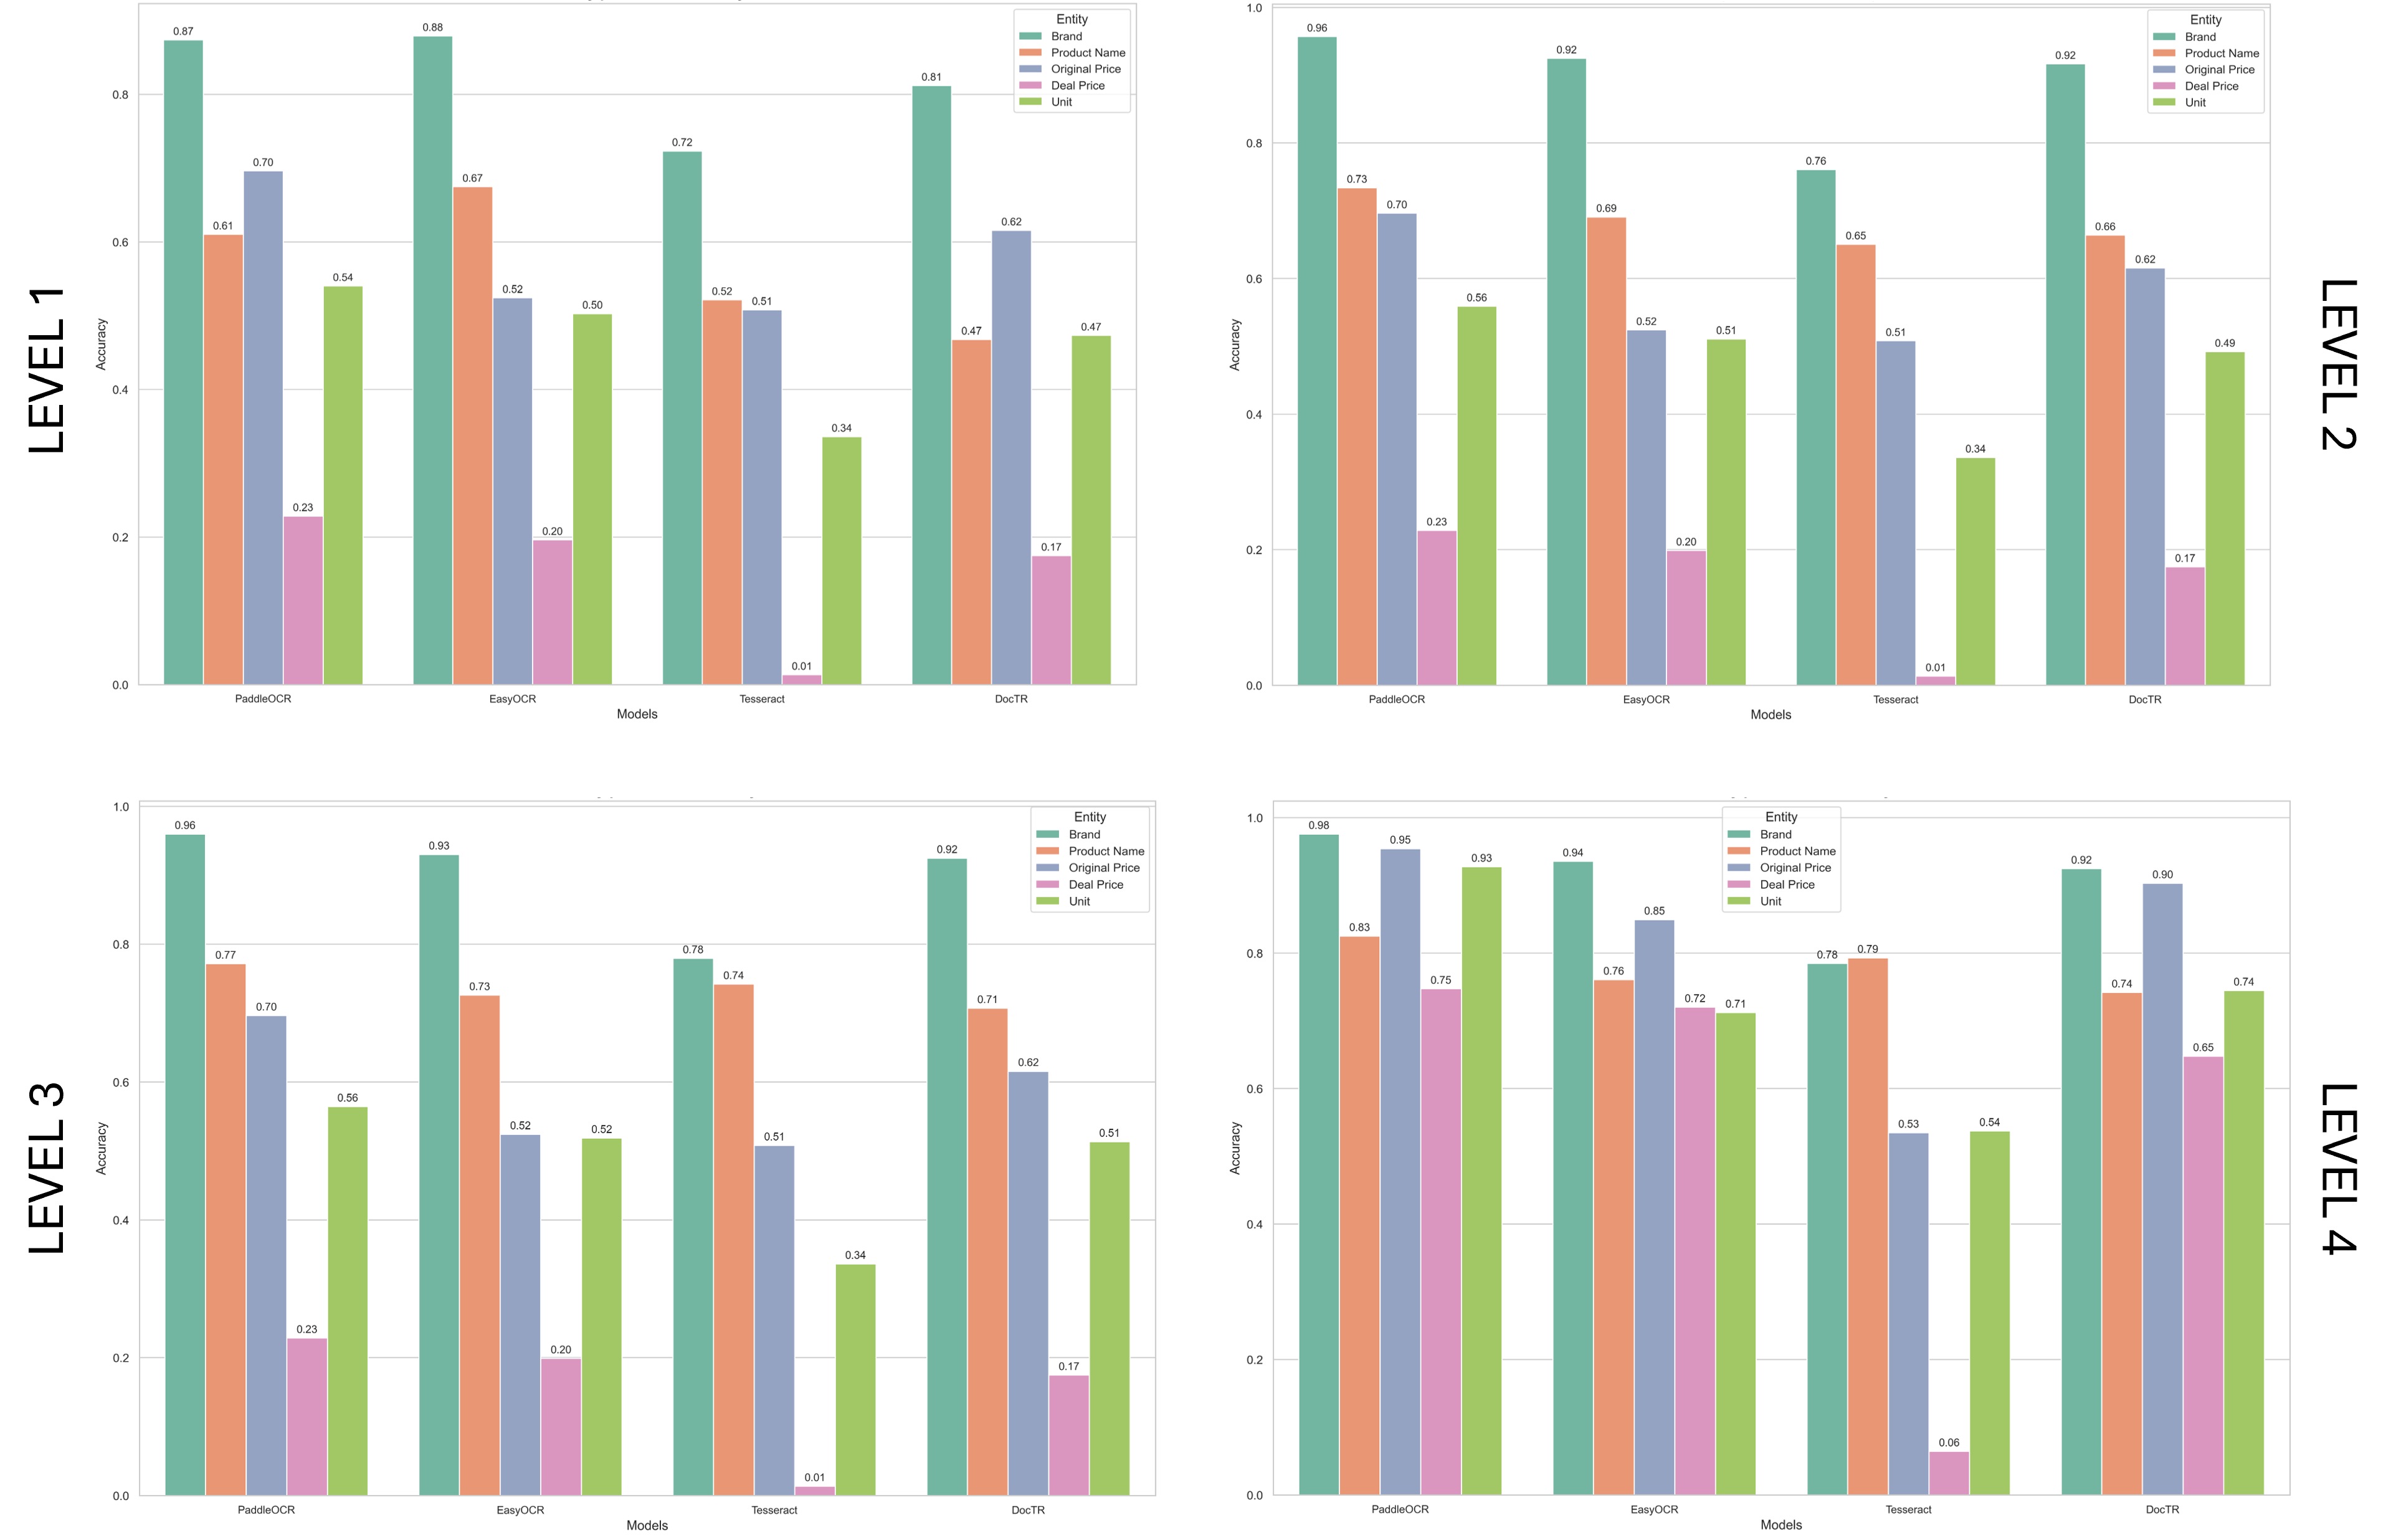
\includegraphics[width=0.8\linewidth]{figures/eval_ocr_accuracies.png}
    \caption{Accuracy per Entity of OCR Models at Different Normalization Levels.}
    \label{fig:eval_ocr_accuracies}
\end{figure*}

In general, the OCR models exhibit superior performance in extracting words compared to numerical values. This discrepancy is particularly evident in entity-wise accuracy variations. At the baseline level (normalization level 1), the deal price entity consistently shows the lowest accuracy, whereas the brand entity achieves the highest. The accuracy of other entities varies significantly, with PaddleOCR, EasyOCR, and docTR displaying comparable performance, while Tesseract lags behind.

The overall accuracy improves with increasing normalization levels, with normalization level 4 yielding the highest accuracy gains. At this level, Tesseract continues to struggle with deal price recognition, failing in over 90\% of cases. In contrast, the other OCR models achieve accuracies exceeding 70\% across nearly all entity types.

Among the different entities, brand names are consistently recognized with the highest accuracy. This can be attributed to their simpler linguistic structure and distinct visual presentation, as brand names are often bolded or highlighted in promotional material. In contrast, product names tend to have more complex linguistic structures, making exact string matching more challenging.

The recognition of unit information lags behind brand names but remains more accurate than deal prices. The reduced accuracy can be explained by the smaller font size of unit labels, their less prominent placement, and the high variability in unit measurements (e.g., "kg", "g", "Stück"), which complicates recognition.

A significant gap is observed between deal price and original price accuracy. This can be attributed to the typographic differences between the two: deal prices are often emphasized using distinctive fonts and superscripted decimals, making them harder for OCR models to interpret correctly. In contrast, original prices are typically displayed in a standard inline format, which is easier to recognize.

\begin{figure*}[h!]
    \centering
    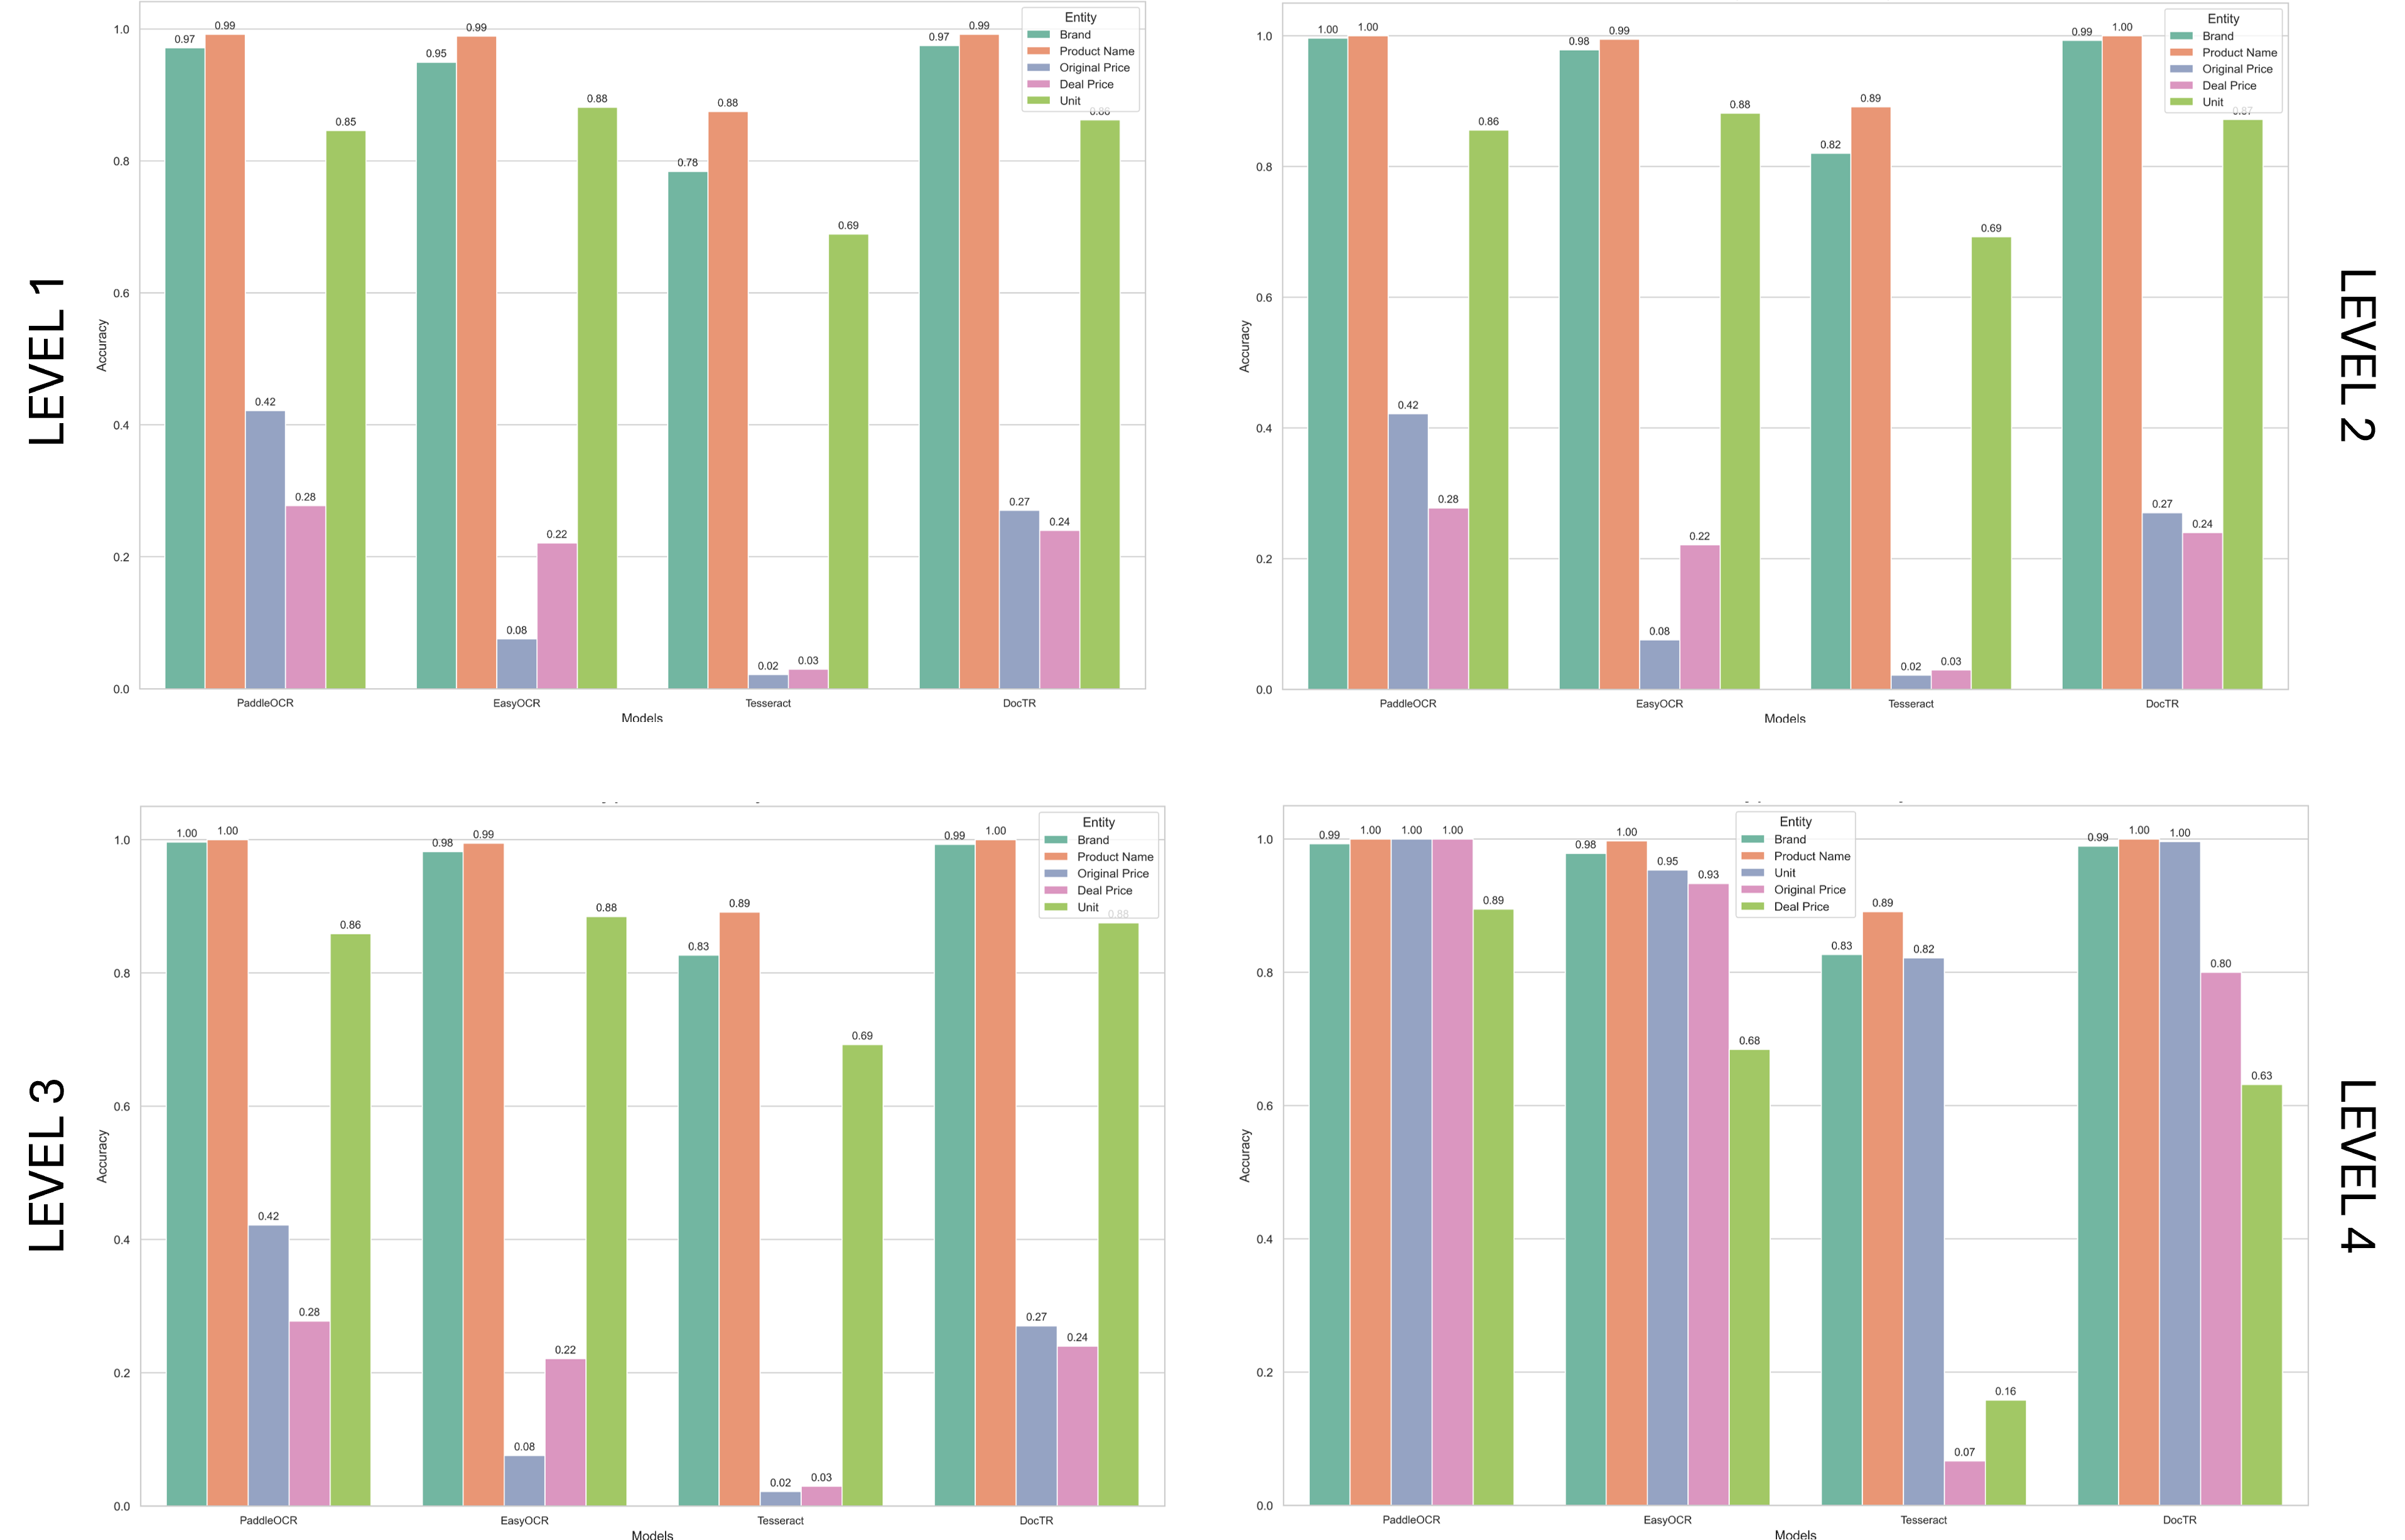
\includegraphics[width=0.8\linewidth]{figures/eval_ocr_ngram_accuracies.png}
    \caption{N-gram Accuracy per Entity of OCR Models at Different Normalization Levels.}
    \label{fig:eval_ocr_ngram_accuracies}
\end{figure*}

When evaluating n-gram accuracy per-entity in \figref{fig:eval_ocr_ngram_accuracies}, the results reveal a similar trend to per-entity accuracy. When comparing the OCR models, PaddleOCR consistently outperforms the other models especially in the price extractions while Tesseract lacks behind in all entities.

The most significant observation is that the deal price and original price exhibit in lower normalization levels significantly worse accuracies. Since the length of n-gram sequences increase superlinearly, longer entity values, precisely the brand and product name, more likely achieve higher accuracies, which is also reflected in the results.

At the highest normalization level, most models achieve 100\% or close to 100\% n-gram accuracy in the majority of entites. Additionally, here the discrepancy of Tesseract is most visible, where it cannot nearly achieve comparable scores. Also, one can observe that the unit entity drops significantly at level 4 across all models. This can be attributed to the high variability in unit measurements, which makes it challenging to match the exact n-grams.

%TODO: Add table with entity-avg results

% EXPERIMENT: OCR+LLM
\subsubsection{Hybrid-OCR+LLM Performance}

In addition to evaluating the OCR capabilities, the performance of OCR models was assessed in conjunction with large language models (LLMs). The primary questions addressed were:
\begin{itemize}
    \item Which LLM is best suited to work with these OCR outputs?
    \item Which OCR and LLM combination works best for information extraction (IE)?
\end{itemize}

All 372 samples of the Leaflet-IE dataset were used for evaluation. It is assumed that neither the OCR models nor the LLMs have previously encountered this data, similar to the OCR evaluation. Since the task is to extract structured information, the evaluation metrics were adapted to reflect the performance of the OCR-LLM combination in generating key-value mappings. The evaluation metrics include:
\begin{itemize}
    \item \textbf{Accuracy (Per Entity):} Measures the accuracy (of each extracted entity).
    \item \textbf{Levenshtein Distance:} Calculates the distance between the prediction and the ground truth.
\end{itemize}

The LLMs were prompted to extract entities from the OCR output. The specific prompt used can be found in the appendix (see Appendix \ref{appendix:prompt}).

\paragraph{Models Evaluated:}
\begin{itemize}
    \item \textbf{Llama 3.1 [8b, Q4]}: \texttt{llama3.1\_8b},
    \item \textbf{Qwen 2.5 [1.5b, Q8]}: \texttt{qwen2.5\_1.5b-instruct-q8\_0},
    \item \textbf{Llama 3.2 [3b, Q8]}: \texttt{llama3.2\_3b-instruct-q8\_0},
    \item \textbf{Qwen 2.5 [7b, Q4]}: \texttt{qwen2.5\_7b},
\end{itemize}
where the LLM name and version is additionally specified through the model size (in billions of parameters) and the quantization level.


To avoid confusion with the normalization used in the OCR experiment, the OCR results were kept raw, as normalization may remove valuable information. The LLMs are expected to handle such inconsistencies and errors in the input. Instead, here the entity values were evaluated in both raw form and with a normalization applied for the comparability between the LLM prediction and the ground truth value . The normalization procedure includes usual character replacements and filtering based on linguistic artifacts commonly encountered in OCR errors. The specific normalization procedure can be found in the appendix 
% TODO: (see Appendix \ref{appendix:ocr_llm_normalization}).

\paragraph{Results:}
The entity-averaged accuracies and Levenshtein distances for the raw OCR output are depicted in Figures \ref{fig:eval_ocr_llm_accuracies_avg} and \ref{fig:eval_ocr_llm_levdist_avg}, respectively.

\begin{figure*}[h!]
    \centering
    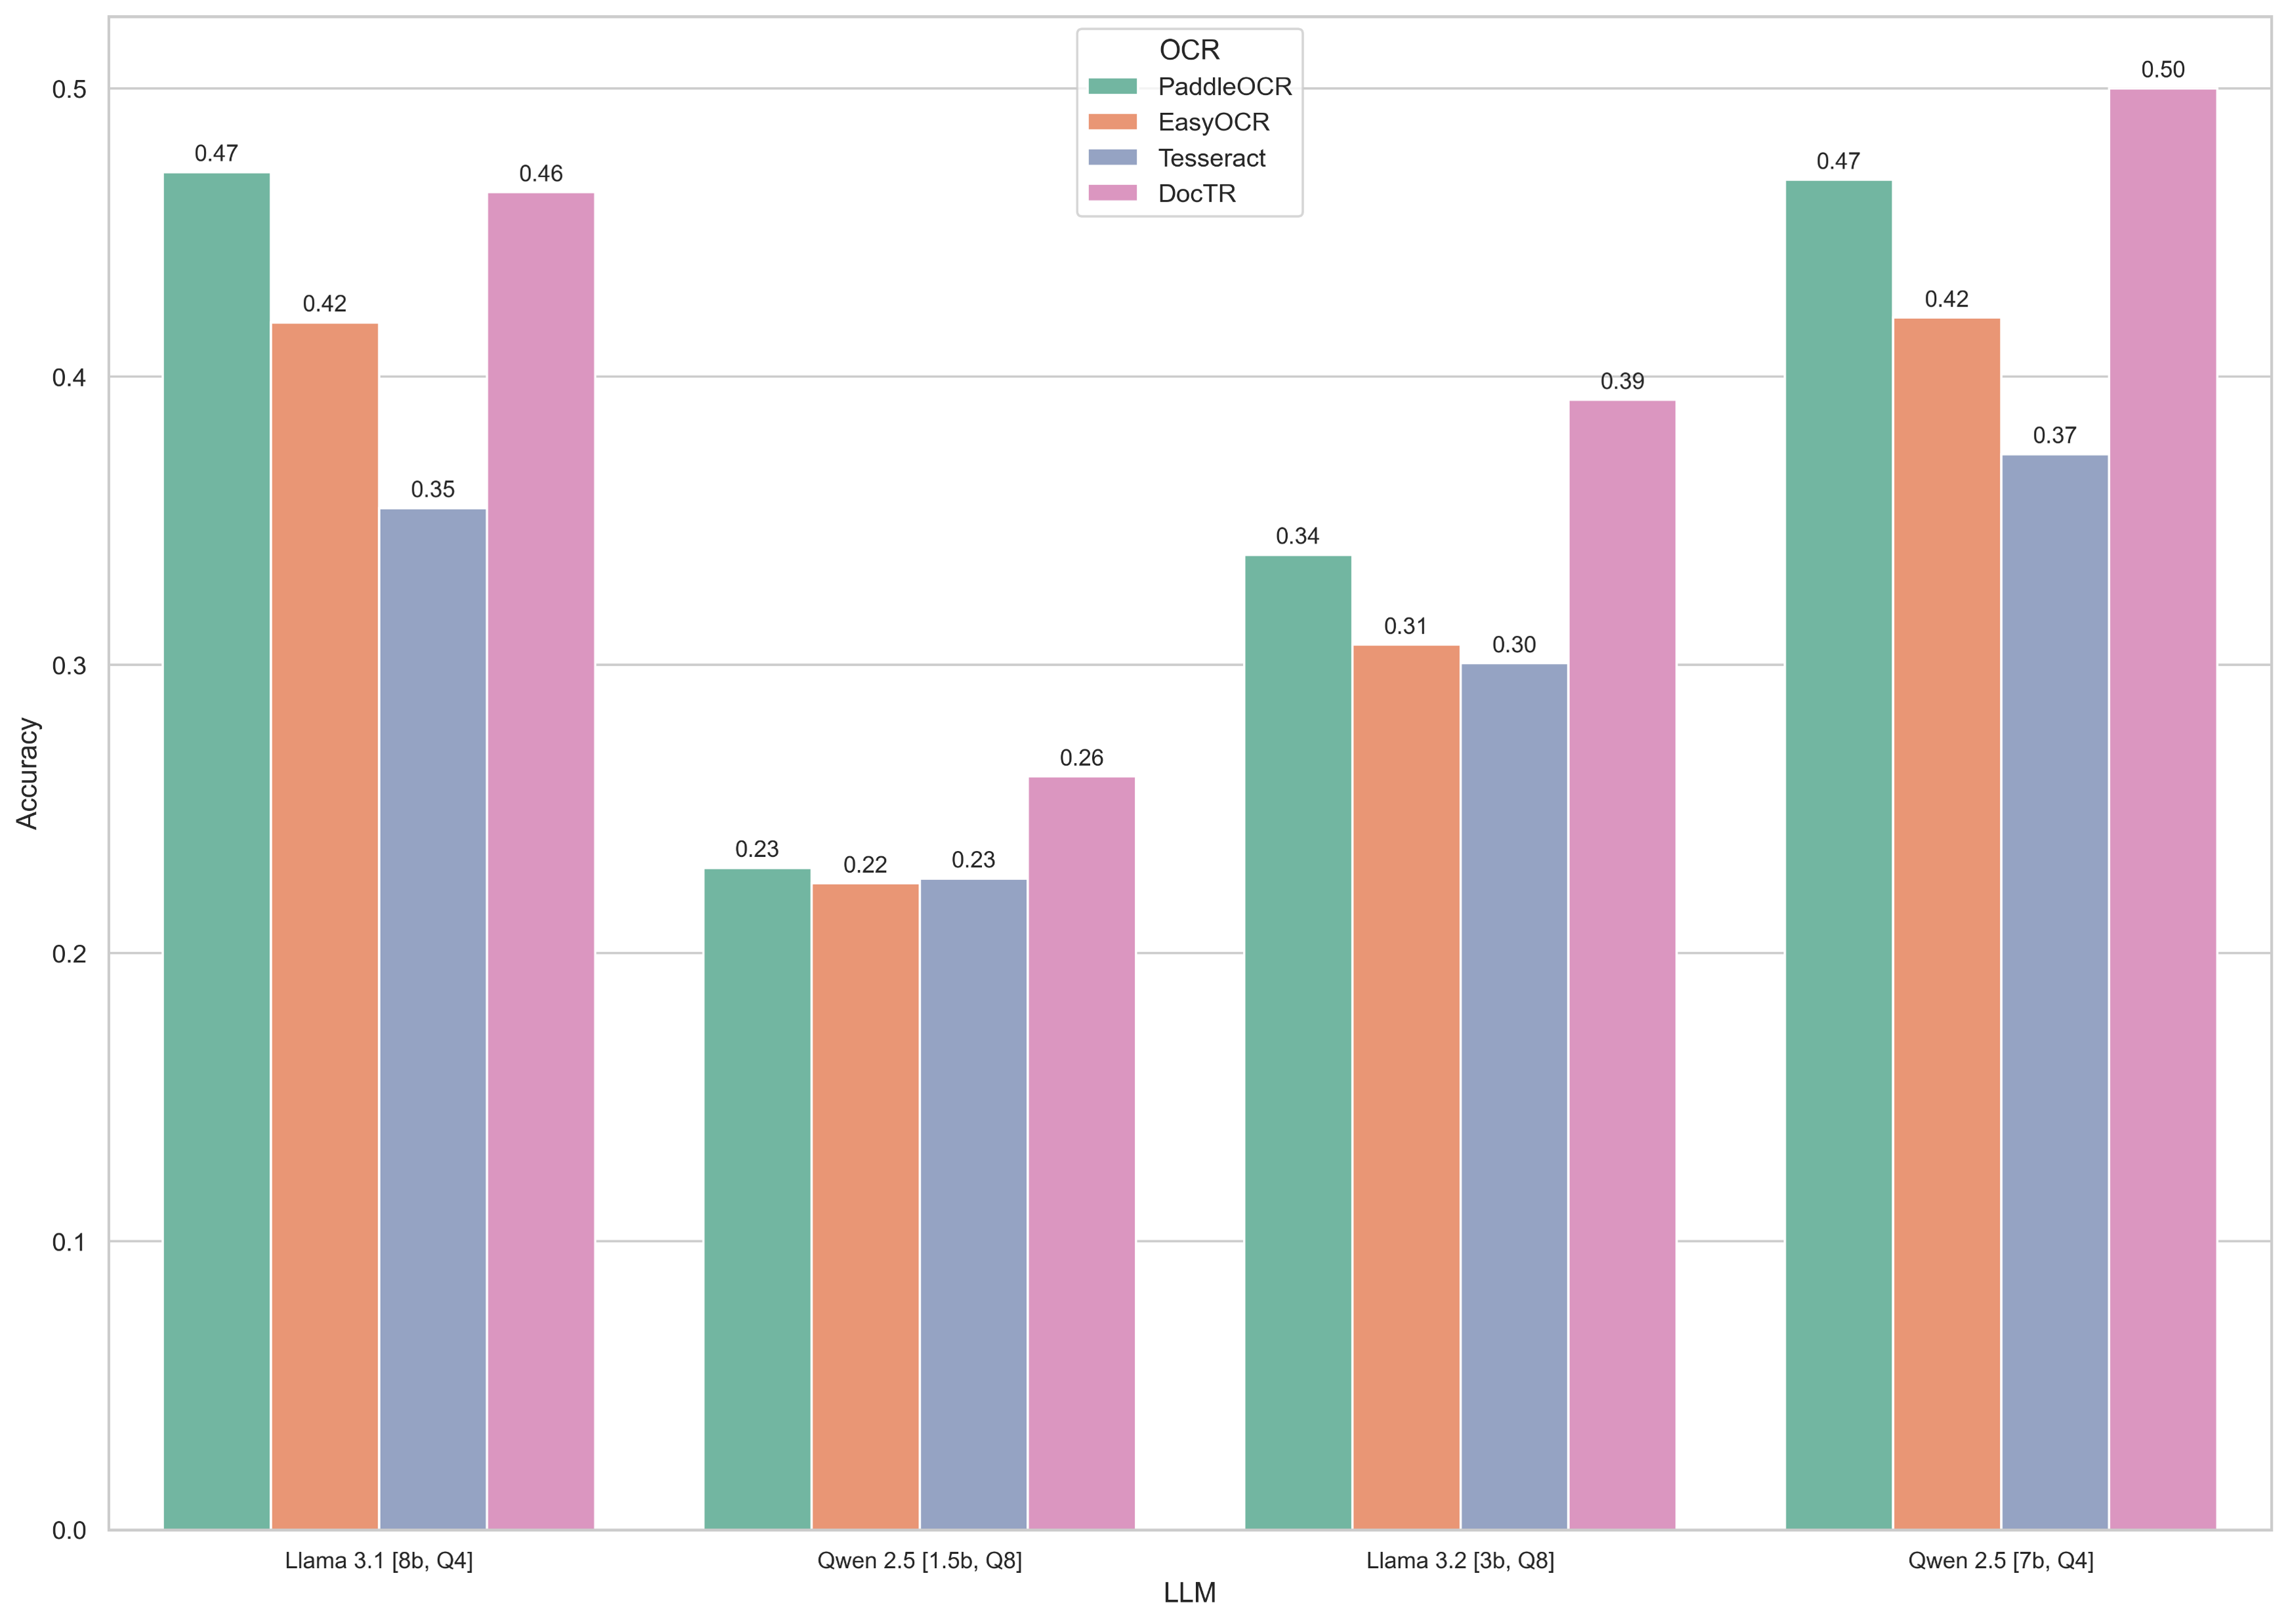
\includegraphics[width=0.8\linewidth]{figures/eval_ocr_llm_accuracies_avg.png}
    \caption{Entity-Averaged Accuracy of LLM Models per Raw OCR Output.}
    \label{fig:eval_ocr_llm_accuracies_avg}
\end{figure*}

The averaged accuracies reveal that a higher number of parameters is more beneficial for the LLMs in this task than a higher quantization level. Specifically, the Llama 3.1:8b and Qwen 2.5:7b models achieve significantly higher accuracy scores than their counterparts with a lower number of parameters. Qwen 2.5:1.5b in Q8 performs worse than Llama 3.2:3b in Q8, but Qwen 2.5:7b in Q4 is overall the best. These differences can be attributed to multiple factors, such as the pre-training data of the models, the model architecture, or the prompt used to extract the entities. DocTR and PaddleOCR achieve equal or better results than Tesseract and EasyOCR. Specifically, Tesseract consistently performs the worst among the evaluated models.


% \begin{figure*}[h!]
%     \centering
%     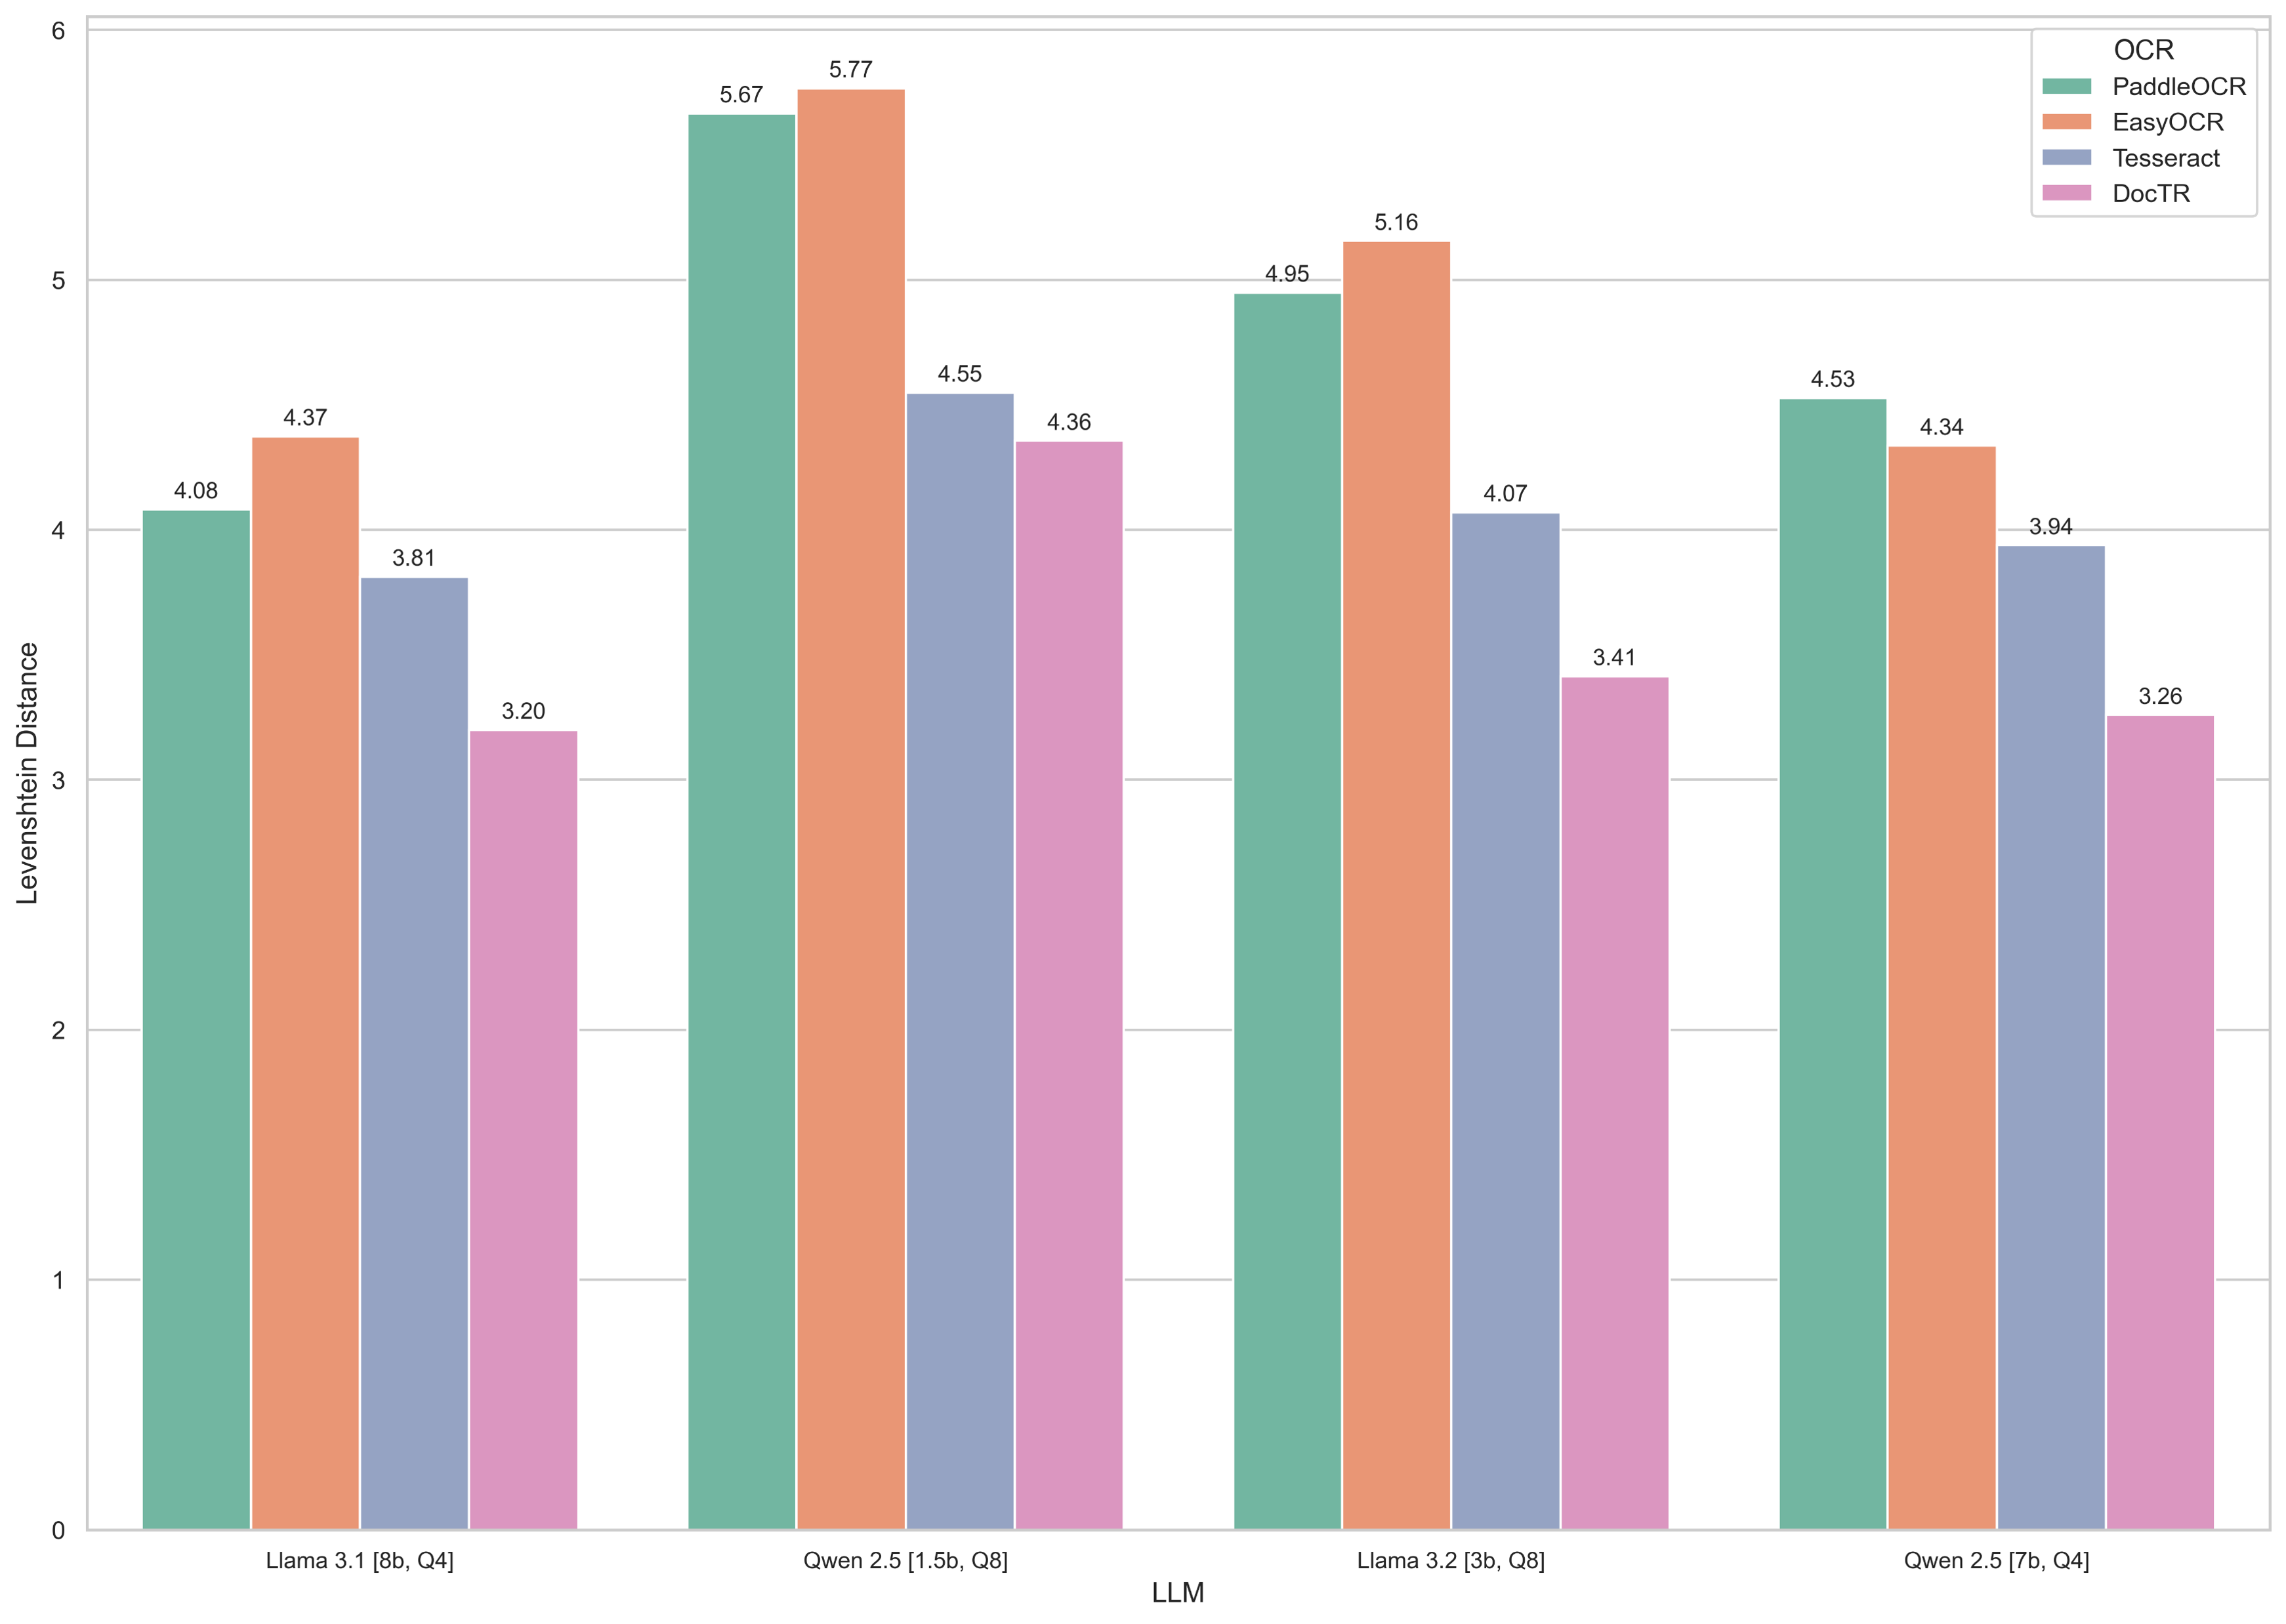
\includegraphics[width=0.8\linewidth]{figures/eval_ocr_llm_levdist_avg.png}
%     \caption{Entity-Averaged Levenshtein Distance of OCR-LLM Models (Raw OCR Output).}
%     \label{fig:eval_ocr_llm_levdist_avg}
% \end{figure*}
% FIGURE TWO COLUMNS WIDE
\begin{figure*}[h!]
    \centering
    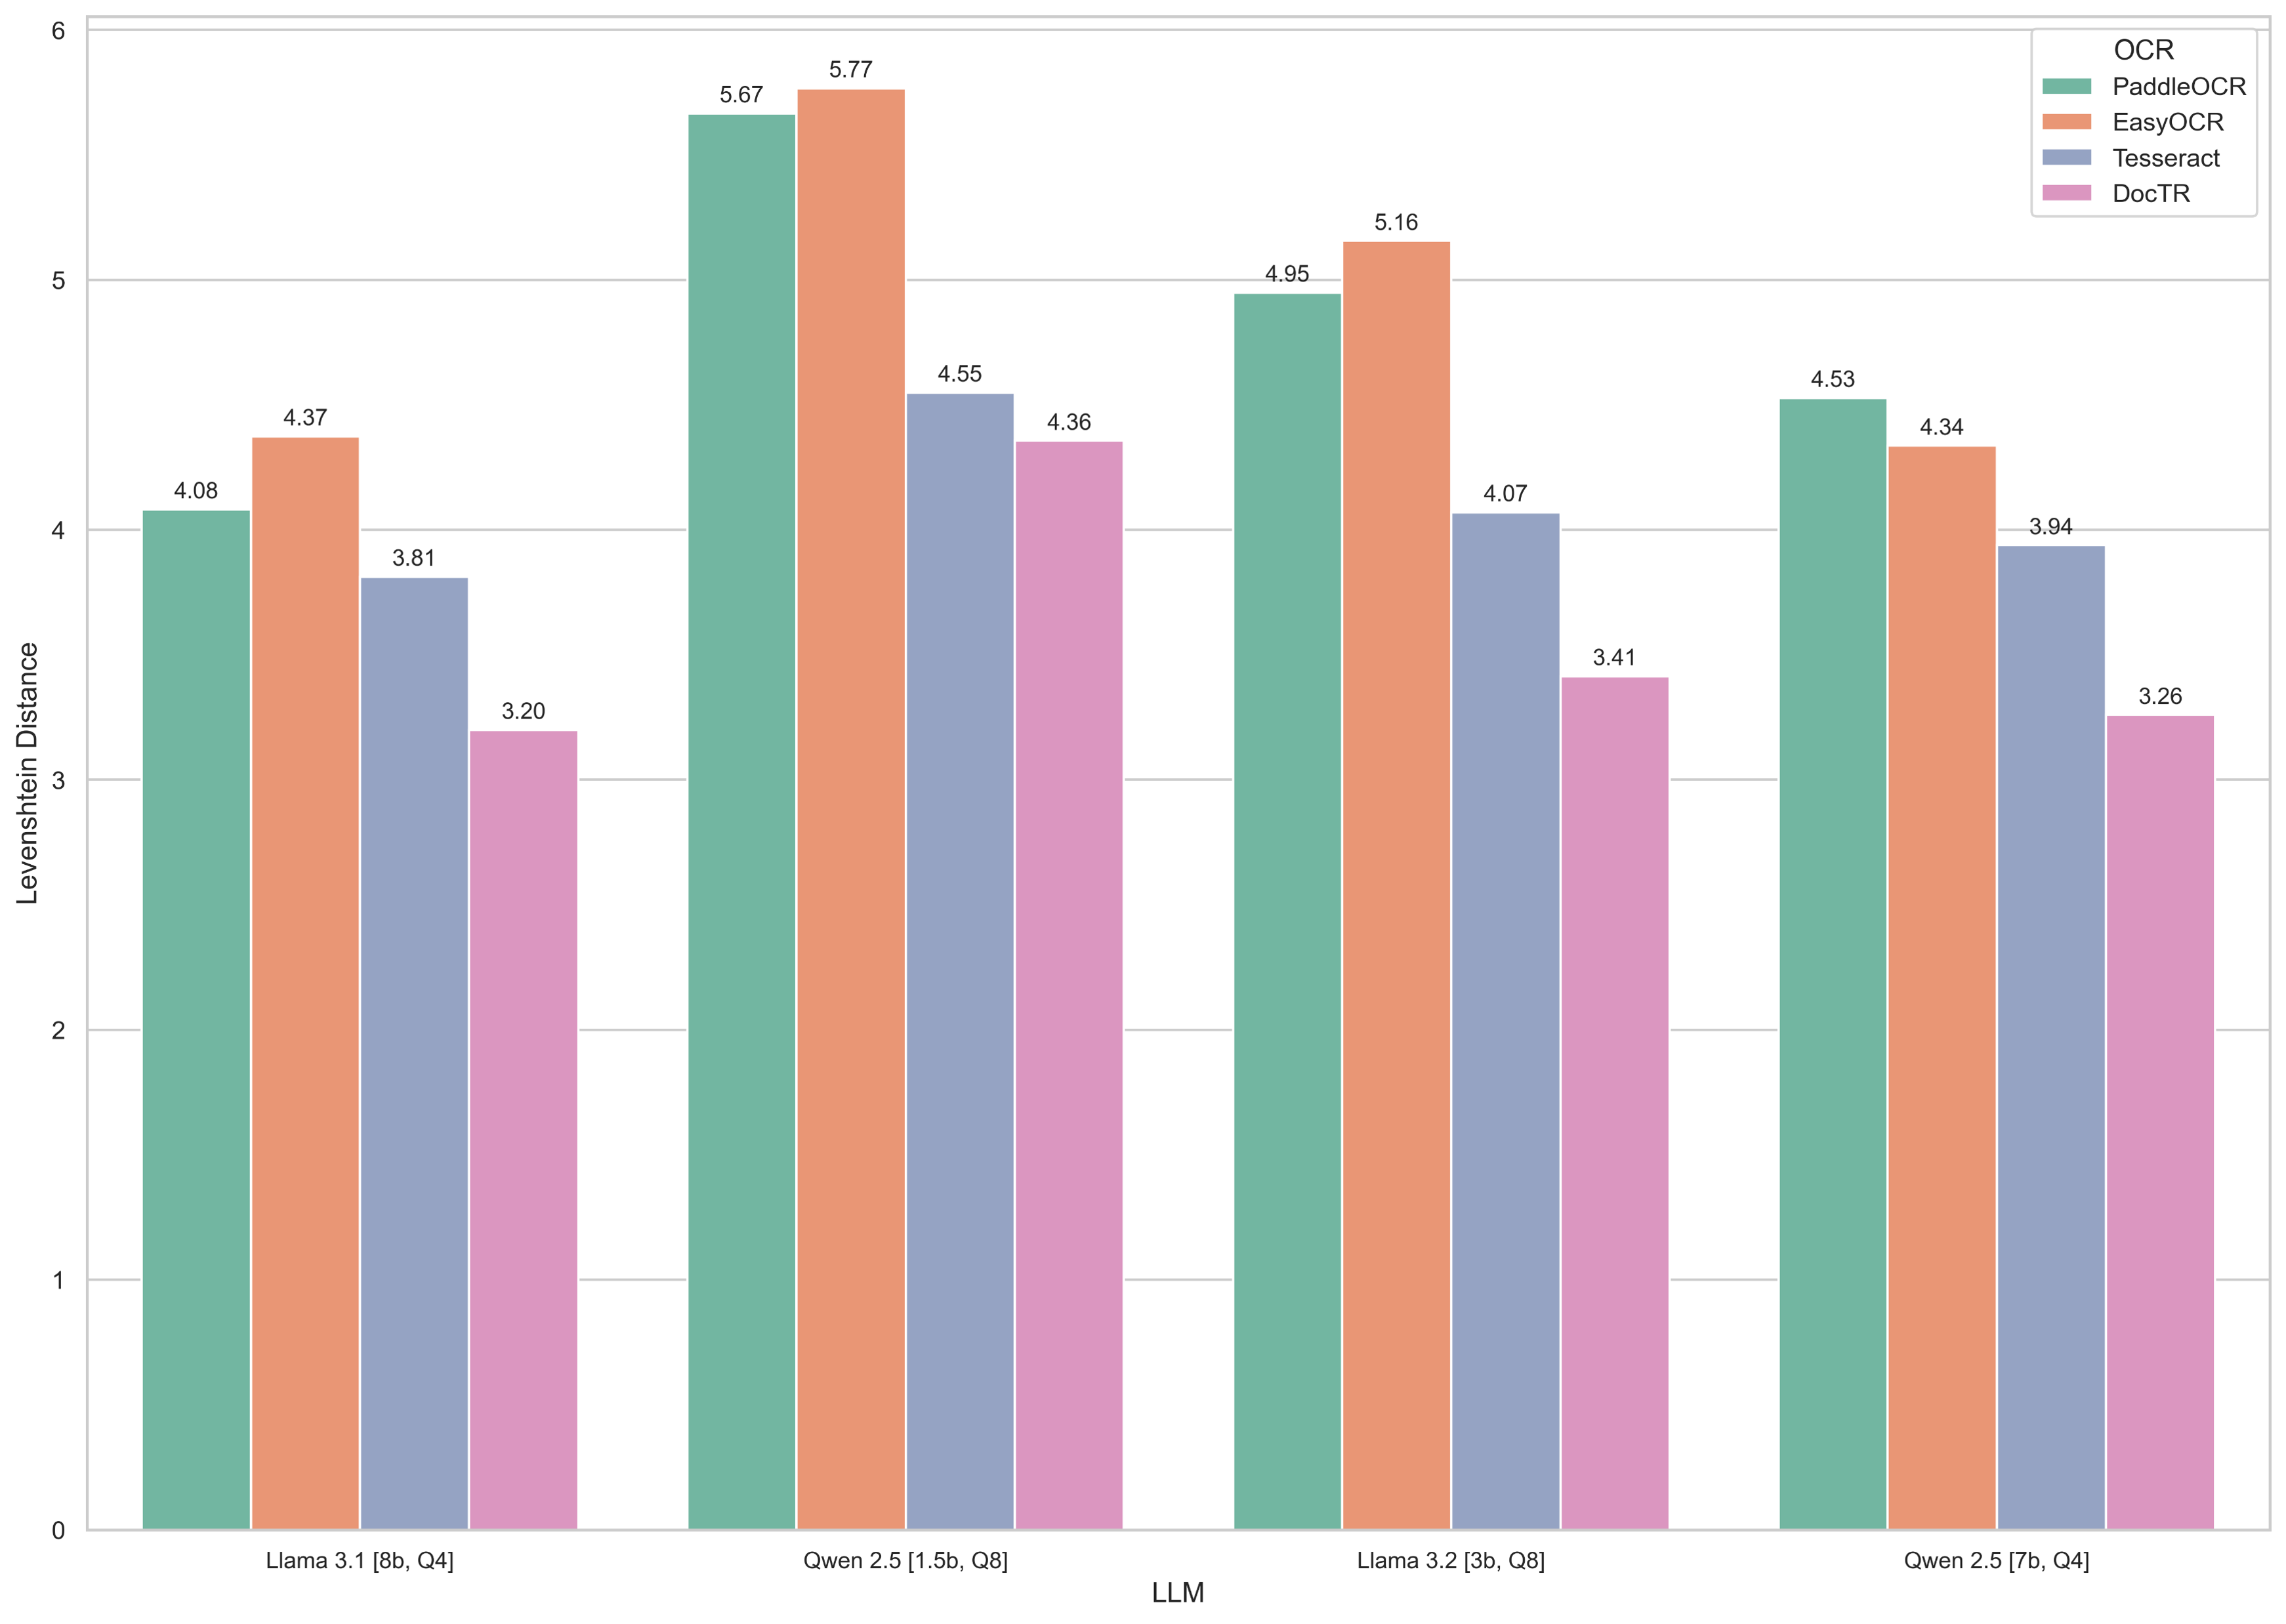
\includegraphics[width=0.7\linewidth]{figures/eval_ocr_llm_levdist_avg.png}
    \caption{Entity-Averaged Levenshtein Distance of OCR-LLM Models (Raw OCR Output).}
    \label{fig:eval_ocr_llm_levdist_avg}
\end{figure*}

When regarding the levenshtein distances, the results show similar trends. DocTR delivers by far the best OCR input across all OCR models. Suprisingly, Tesseract achieves lower levenshtein distances than PaddleOCR and EasyOCR, with EasyOCR being the worst across all models. This could be due to the fact that Tesseract delivers more often slightly wrong but still similar results, while EasyOCR delivers less often wrong but more different results. The LLMs show similar trends as in the accuracy evaluation, but Llama 3.1:8b now slightly outperforms Qwen 2.5:7b. The differences between the LLMs are less pronounced than in the accuracy evaluation, which can be attributed to the unnormalized levenshtein distance calculation used.

% The entity-specific accuracies for the raw OCR output are shown in \figref{fig:eval_ocr_llm_accuracies_raw}, while the entity-specific levenshtein distances for the raw OCR output are shown in \figref{fig:eval_ocr_llm_levenshtein_raw}.

% \begin{figure*}[h!]
%     \centering
%     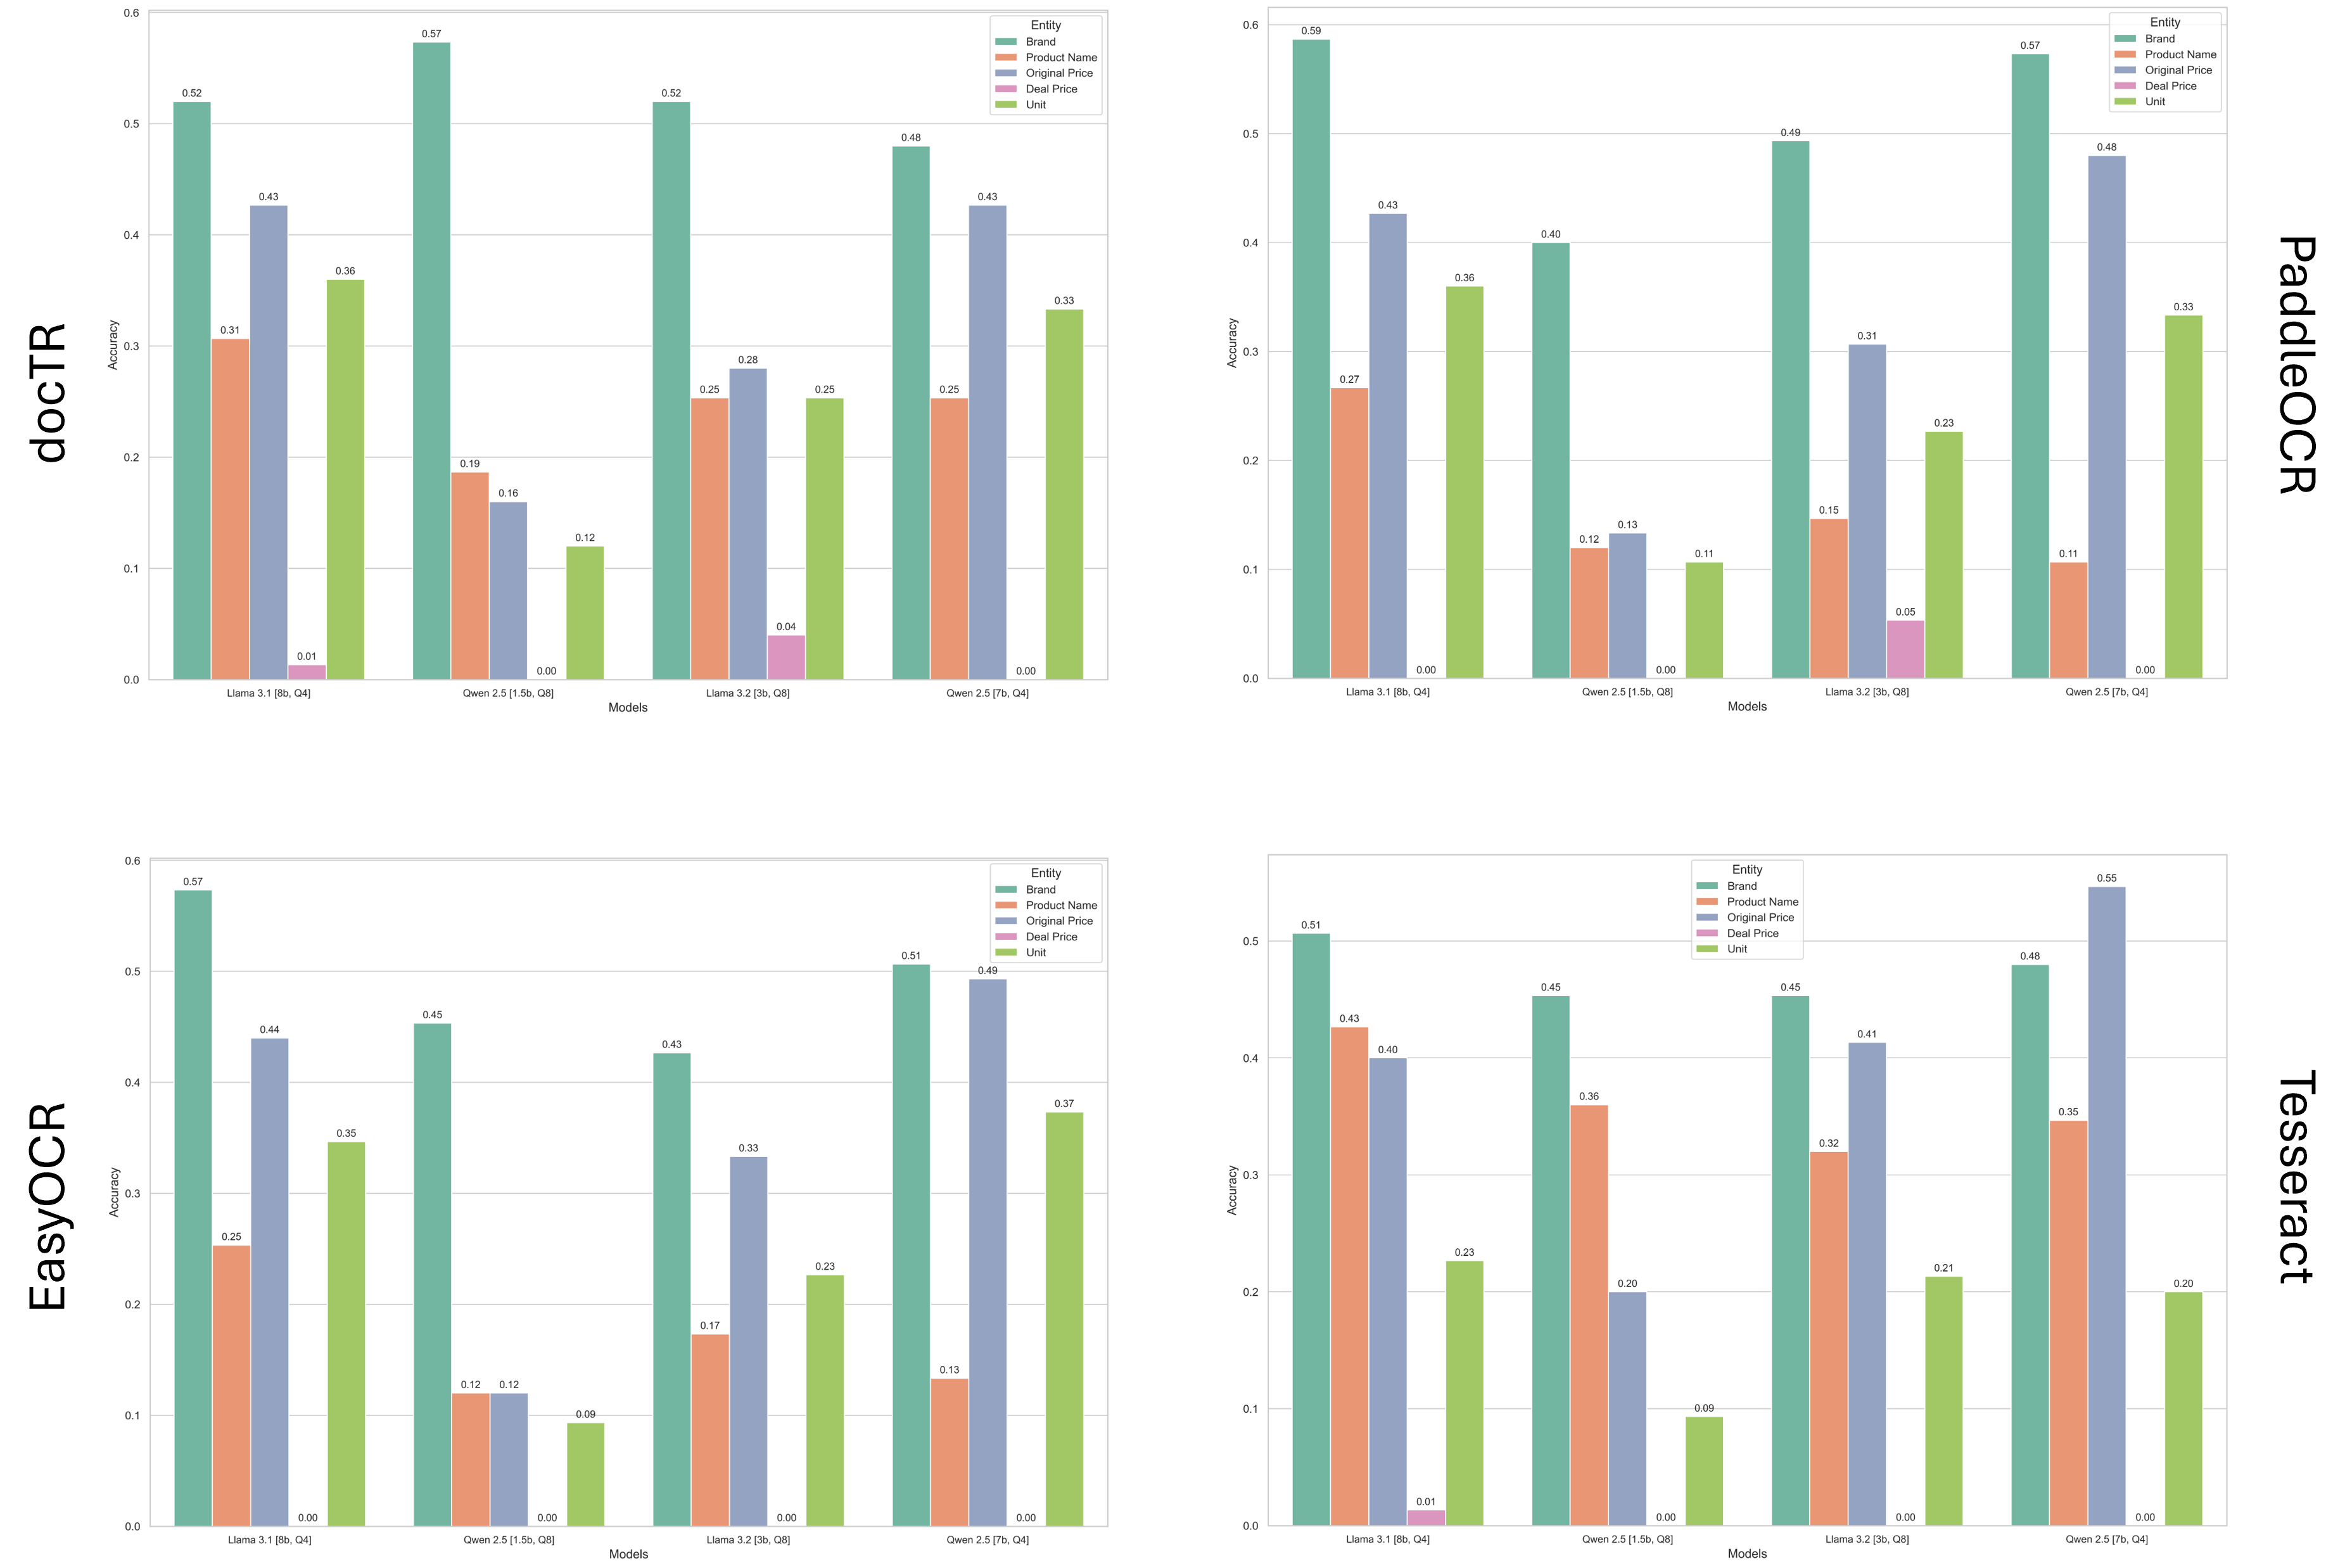
\includegraphics[width=0.8\linewidth]{figures/eval_ocr_llm_accuracies_raw.png}
%     \caption{Accuracy per Entity of OCR-LLM Models (Raw OCR Output).}
%     \label{fig:eval_ocr_llm_accuracies_raw}
% \end{figure*}

% \begin{figure*}[h!]
%     \centering
%     \includegraphics[width=0.8\linewidth]{figures/eval_ocr_llm_accuracies_normalized.png}
%     \caption{Accuracy per Entity of OCR-LLM Models (Normalized OCR Output).}
%     \label{fig:eval_ocr_llm_accuracies_normalized}
% \end{figure*}

% \begin{figure*}[h!]
%     \centering
%     \includegraphics[width=0.8\linewidth]{figures/eval_ocr_llm_levenshtein_raw.png}
%     \caption{Levenshtein Distance per Entity of OCR-LLM Models (Raw OCR Output).}
%     \label{fig:eval_ocr_llm_levenshtein_raw}
% \end{figure*}

% \begin{figure*}[h!]
%     \centering
%     \includegraphics[width=0.8\linewidth]{figures/eval_ocr_llm_levenshtein_normalized.png}
%     \caption{Levenshtein Distance per Entity of OCR-LLM Models (Normalized OCR Output).}
%     \label{fig:eval_ocr_llm_levenshtein_normalized}
% \end{figure*}


\subsection{Donut Fine-Tuning Performance}
Experiment Question:
- Is it possible to train a Vision Encoder Decoder model to extract end2end information from supermarket leaflet deal images?

Setup:

Results:






% \subsection{Comparison of Hybrid OCR+LLM, Donut, and LVLM}
% - Evaluating the results from the prepending experiments, the main goal is to compare the performance of the best OCR + LLM model with end-to-end models.
% - As best OCR + LLM model, the decision was made to use DocTR as OCR model and Qwen 2.5:7b as well as Llama 3.1:8b as LLM models due to their similar performance.
% - Donut was used as end-to-end Vision Encoder Decoder Model
% - As LVLMs, MiniCPM-V and Llama3.2-Vision were used.

% - Dataset: Leaflet-IE validation subset, since Donut was trained on the train subset.
% - Evaluation Metrics: Accuracy, levenshtein distance on entity level
% - Normalization: The same approach as in OCR + LLM evaluation was used to normalize the entity value predictions and the corresponding ground truth values.


% \indent{\textbf{Results}.}
% - Per-Entity Accuracy without normalization (\figref{fig:eval_final_acc_raw})
%     - OCR+LLM significantly worst, on validation subset original and deal price at 0\% accuracy
%     - LVLM by far the best, especially in deal price. This is because LVLMs are able to use spatial information and context to infer the correct entity values.
%     - Donut can keep up with the LVLMs, but is slightly worse, especially in brand
% - Per-Entity Levenshtein Distance without normalization (\figref{fig:eval_final_levdis_raw})
%     - LVLMs and donut overall very low scores, which is expected due to the high accuracy
%     - OCR+LLM much higher scores, Suprisingly especially in brand.
%     - Overall, brand has the highest levenshtein distance, which is uncommon.

% - Per-Entity Accuracy with normalization (\figref{fig:eval_final_acc_norm})
%     - Overall results are much better, especially for OCR+LLM. Here, the price detection is even the best.
%     - But OCR+LLM still significantly worse than LVLMs and Donut.
%     - It is mentionable that Donut achieves very solid and stable accuracies across all entities, whereas the LVLMs have a higher variance.
%     - LVLMs still by fare the best, especially in the prices.
% - Per-Entity Levenshtein Distance with normalization (\figref{fig:eval_final_levdis_norm})
%     - Overall drops in levenshtein distance, especially for OCR+LLM
%     - LVLMs achieve lowest scores, but have high variance
%     - Donut very consistent
%     - Still highest levenshtein distance in brand, which is uncommon.

% Conclusions 
% -> LVLMs are the best choice for IE tasks, especially when spatial information is important. However, LVLMs are very resource-intensive and require a lot of computational power.
% -> Donut is a good alternative, especially when the computational resources are limited. When regarding the limited training resources, it is possible that, in the long run, Donut could outperform the LVLMs in this specific task. It is to mention that models like Donut are very hard to generalize to other tasks, whereas LVLMs can be used for a wide range of tasks.
% -> OCR+LLM is significantly worse. Attributed to the lack of spatial and visual information, error propagation from OCR to LLM, and the lack of training data. However, it is a good choice when computational resources are limited and the task is not too complex.

\subsection{Comparison of Hybrid OCR+LLM, Donut, and LVLM}

This section presents a comparative evaluation of a hybrid OCR+LLM pipeline against end-to-end models, specifically Donut and Large Vision-Language Models (LVLMs), for information extraction (IE) from supermarket leaflets. The assessment focuses on model performance using the best OCR+LLM configuration and two end-to-end approaches.

\subsubsection{Experimental Setup}

\paragraph{Models.} The following models were selected for evaluation:
\begin{itemize}
    \item \textbf{OCR+LLM:} DocTR was utilized as the OCR engine, with Qwen 2.5-7B and LLaMA 3.1-8B serving as LLMs due to their comparable performance.
    \item \textbf{Donut:} An end-to-end Vision Encoder-Decoder model optimized for document understanding.
    \item \textbf{LVLMs:} MiniCPM-V and LLaMA 3.2-Vision were chosen as large vision-language models for comparison.
\end{itemize}

\paragraph{Dataset.} The Leaflet-IE validation subset was used for evaluation since Donut had been trained on the train subset.

\paragraph{Evaluation Metrics.} The models were evaluated using:
\begin{itemize}
    \item \textbf{Accuracy}: The percentage of correctly extracted entity values.
    \item \textbf{Levenshtein Distance}: The edit distance between predicted and ground truth values at the entity level.
\end{itemize}

\paragraph{Normalization.} To ensure consistency, the same normalization approach from the OCR+LLM evaluation was applied to both model predictions and ground truth values.

\subsubsection{Results and Discussion}

\paragraph{Per-Entity Accuracy Without Normalization} (\figref{fig:eval_final_acc_raw})
\begin{itemize}
    \item The OCR+LLM pipeline performed significantly worse than both Donut and LVLMs. Specifically, its accuracy for original and deal price entities was close to 0\%.
    \item LVLMs outperformed all other models, particularly in extracting price-related information. Their superior performance is attributed to their ability to leverage spatial information and contextual cues.
    \item Donut achieved competitive results, closely trailing LVLMs, but showed a notable drop in accuracy for brand recognition.
\end{itemize}

\paragraph{Per-Entity Levenshtein Distance Without Normalization} (\figref{fig:eval_final_levdis_raw})
\begin{itemize}
    \item As expected from the accuracy results, LVLMs and Donut exhibited low Levenshtein distances, indicating high precision.
    \item The OCR+LLM approach had significantly higher edit distances, particularly for brand recognition, suggesting a consistent difficulty in extracting brand names accurately.
    \item Among all entities, brand names showed the highest Levenshtein distance across models, which is uncommon in IE tasks.
\end{itemize}

\paragraph{Per-Entity Accuracy With Normalization} (\figref{fig:eval_final_acc_norm})
\begin{itemize}
    \item Applying normalization significantly improved accuracy, especially for OCR+LLM. Interestingly, its price detection performance exceeded that of Donut in some cases.
    \item Despite the improvements, OCR+LLM remained notably weaker than LVLMs and Donut.
    \item Donut displayed stable and balanced accuracy across all entities, whereas LVLMs exhibited higher variance.
    \item LVLMs retained their leading performance, particularly in price extraction.
\end{itemize}

\paragraph{Per-Entity Levenshtein Distance With Normalization} (\figref{fig:eval_final_levdis_norm})
\begin{itemize}
    \item Levenshtein distances decreased across all models post-normalization, especially for OCR+LLM.
    \item LVLMs achieved the lowest Levenshtein distances but maintained high variance.
    \item Donut demonstrated remarkable consistency across all entities.
    \item The brand entity continued to exhibit the highest Levenshtein distances across models.
\end{itemize}

\subsubsection{Conclusions}

\begin{itemize}
    \item \textbf{LVLMs are the most effective for IE tasks}, particularly when spatial information is crucial. However, their computational requirements are significantly higher, making them less practical in resource-constrained environments.
    \item \textbf{Donut provides a strong trade-off between accuracy and efficiency}. Given the limited training resources, Donut has the potential to outperform LVLMs in the long run for this specific task. However, its generalization ability is limited compared to LVLMs, which can be applied to a wider range of tasks.
    \item \textbf{OCR+LLM is considerably weaker} than the other approaches. Its performance limitations are primarily attributed to:
    \begin{itemize}
        \item Lack of spatial and visual information.
        \item Error propagation from OCR to LLM.
        \item Insufficient training data for robust IE.
    \end{itemize}
    Nevertheless, OCR+LLM remains a viable option when computational resources are constrained, and the task complexity is moderate.
\end{itemize}

\begin{figure*}[h!]
    \centering
    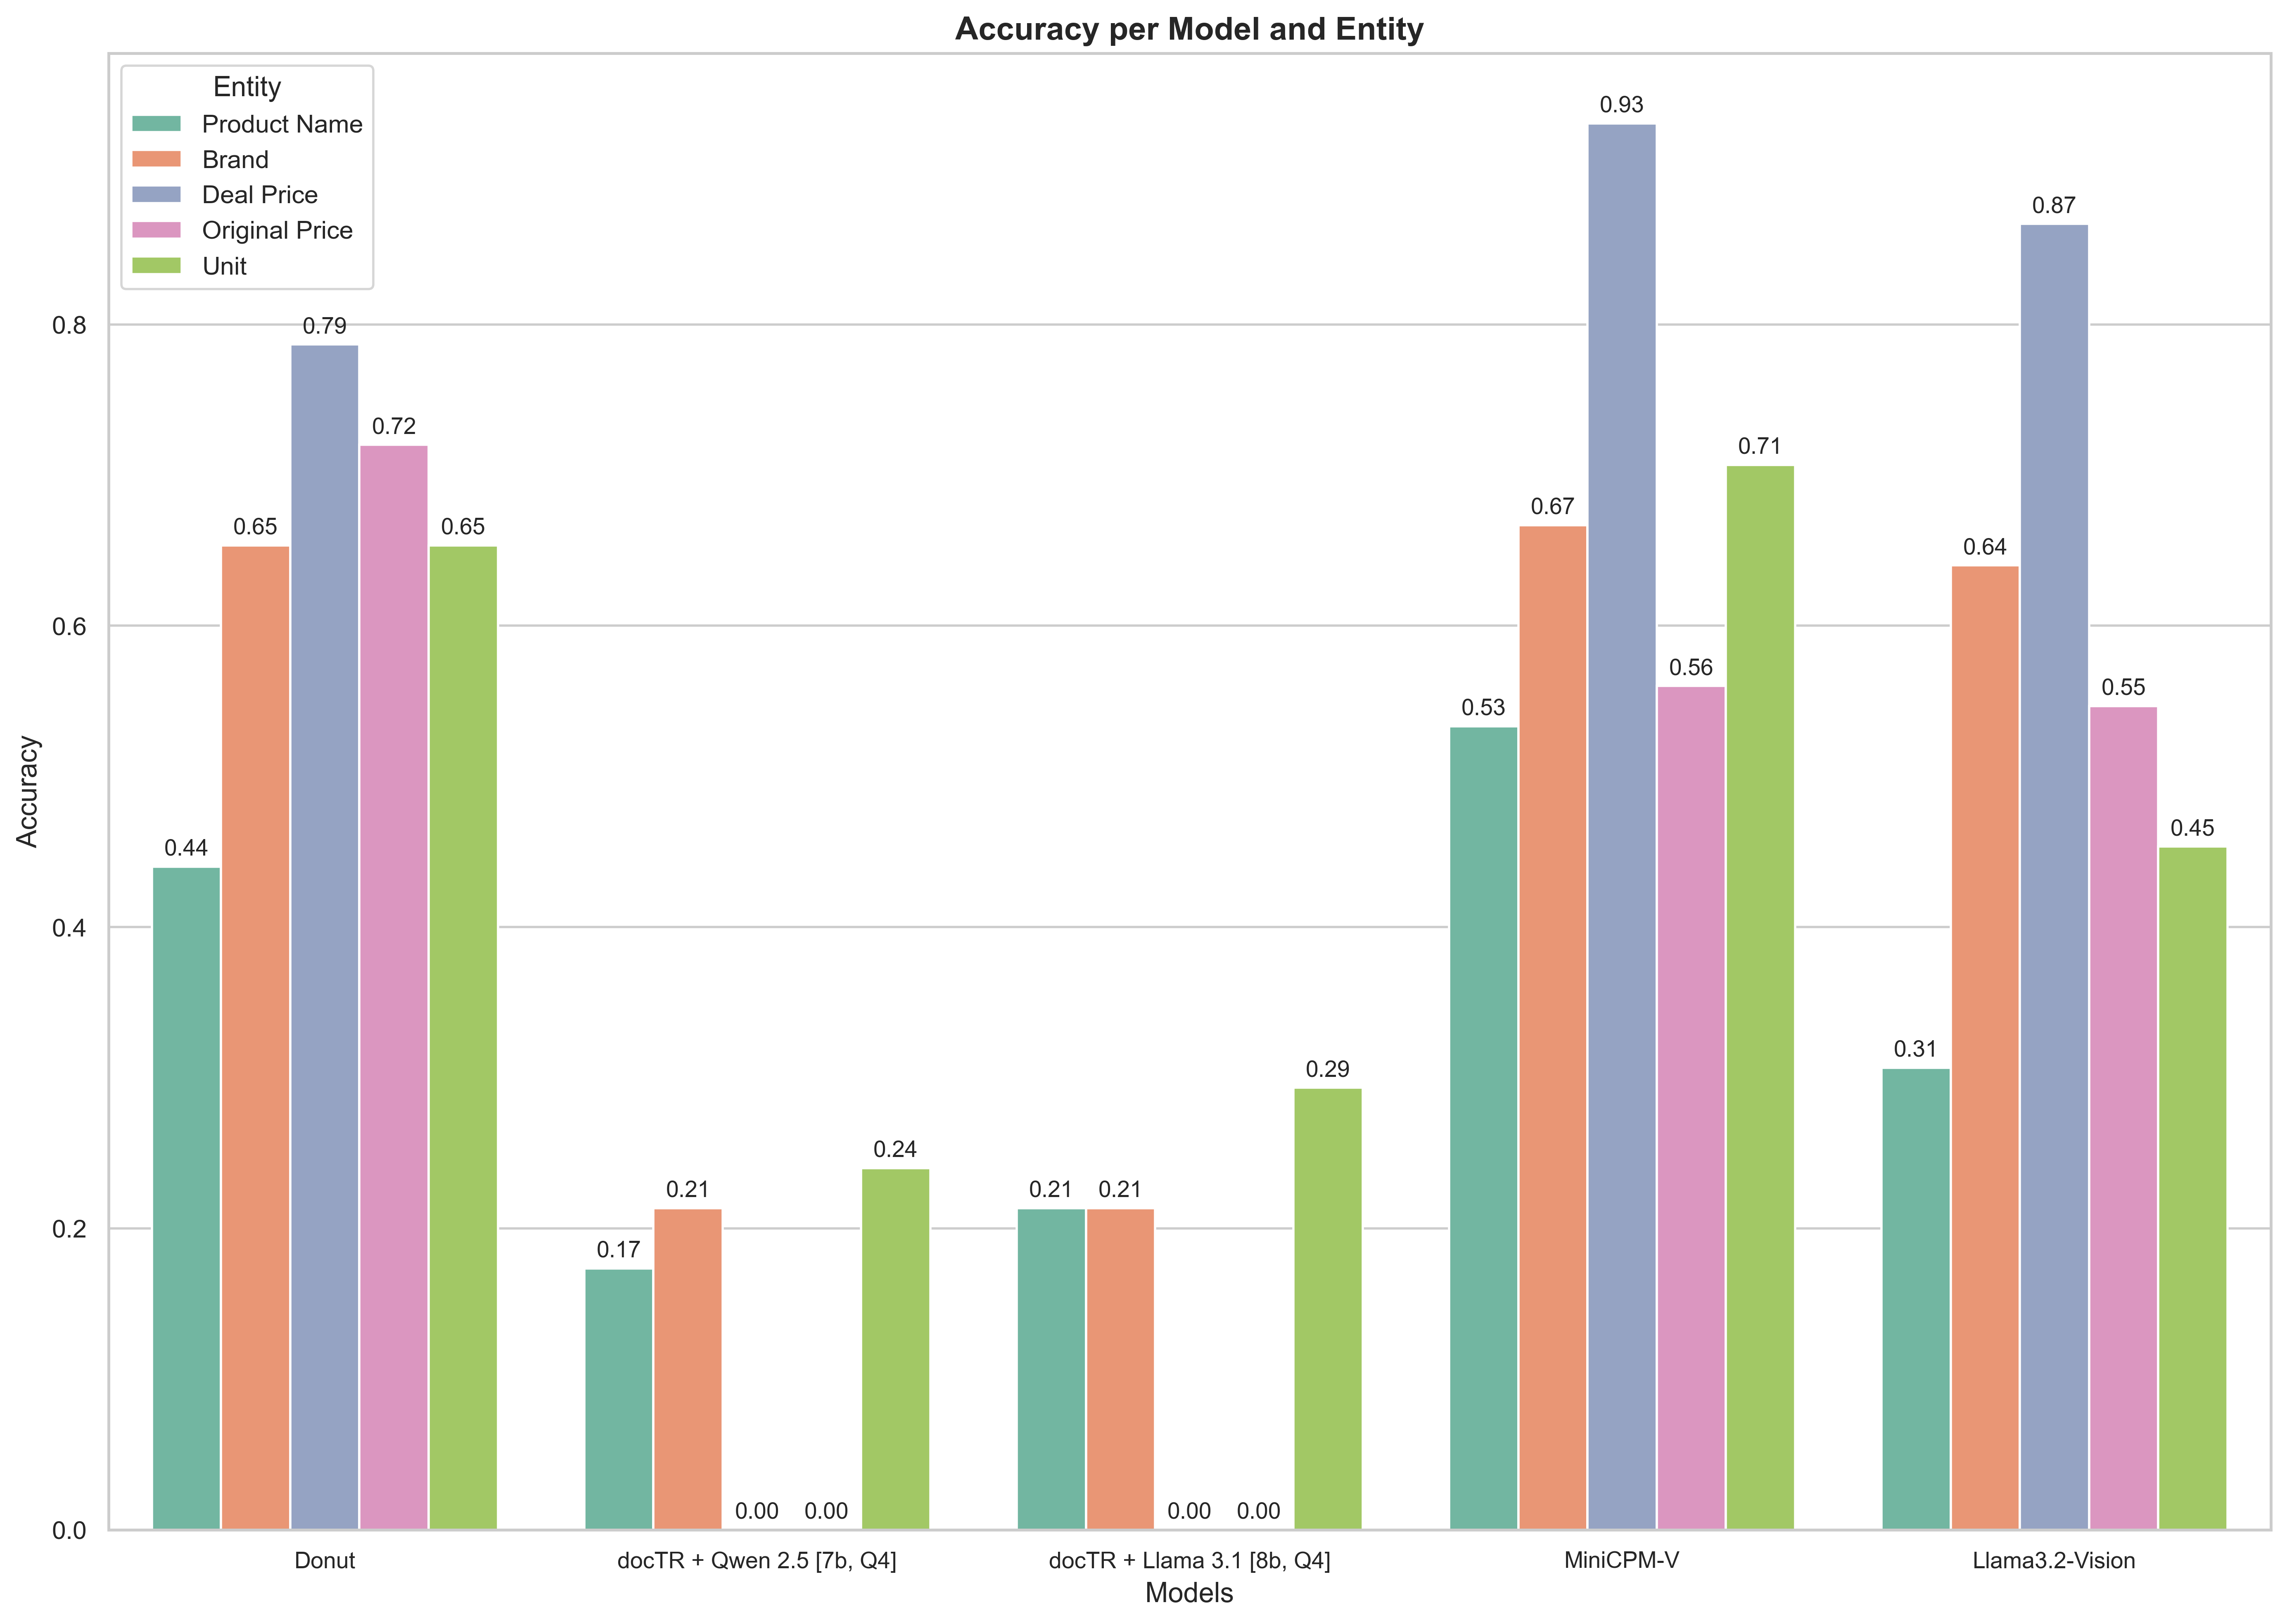
\includegraphics[width=0.8\linewidth]{figures/eval_final_acc_raw.png}
    \caption{Per-Entity Accuracy without normalization.}
    \label{fig:eval_final_acc_raw}
\end{figure*}

\begin{figure*}[h!]
    \centering
    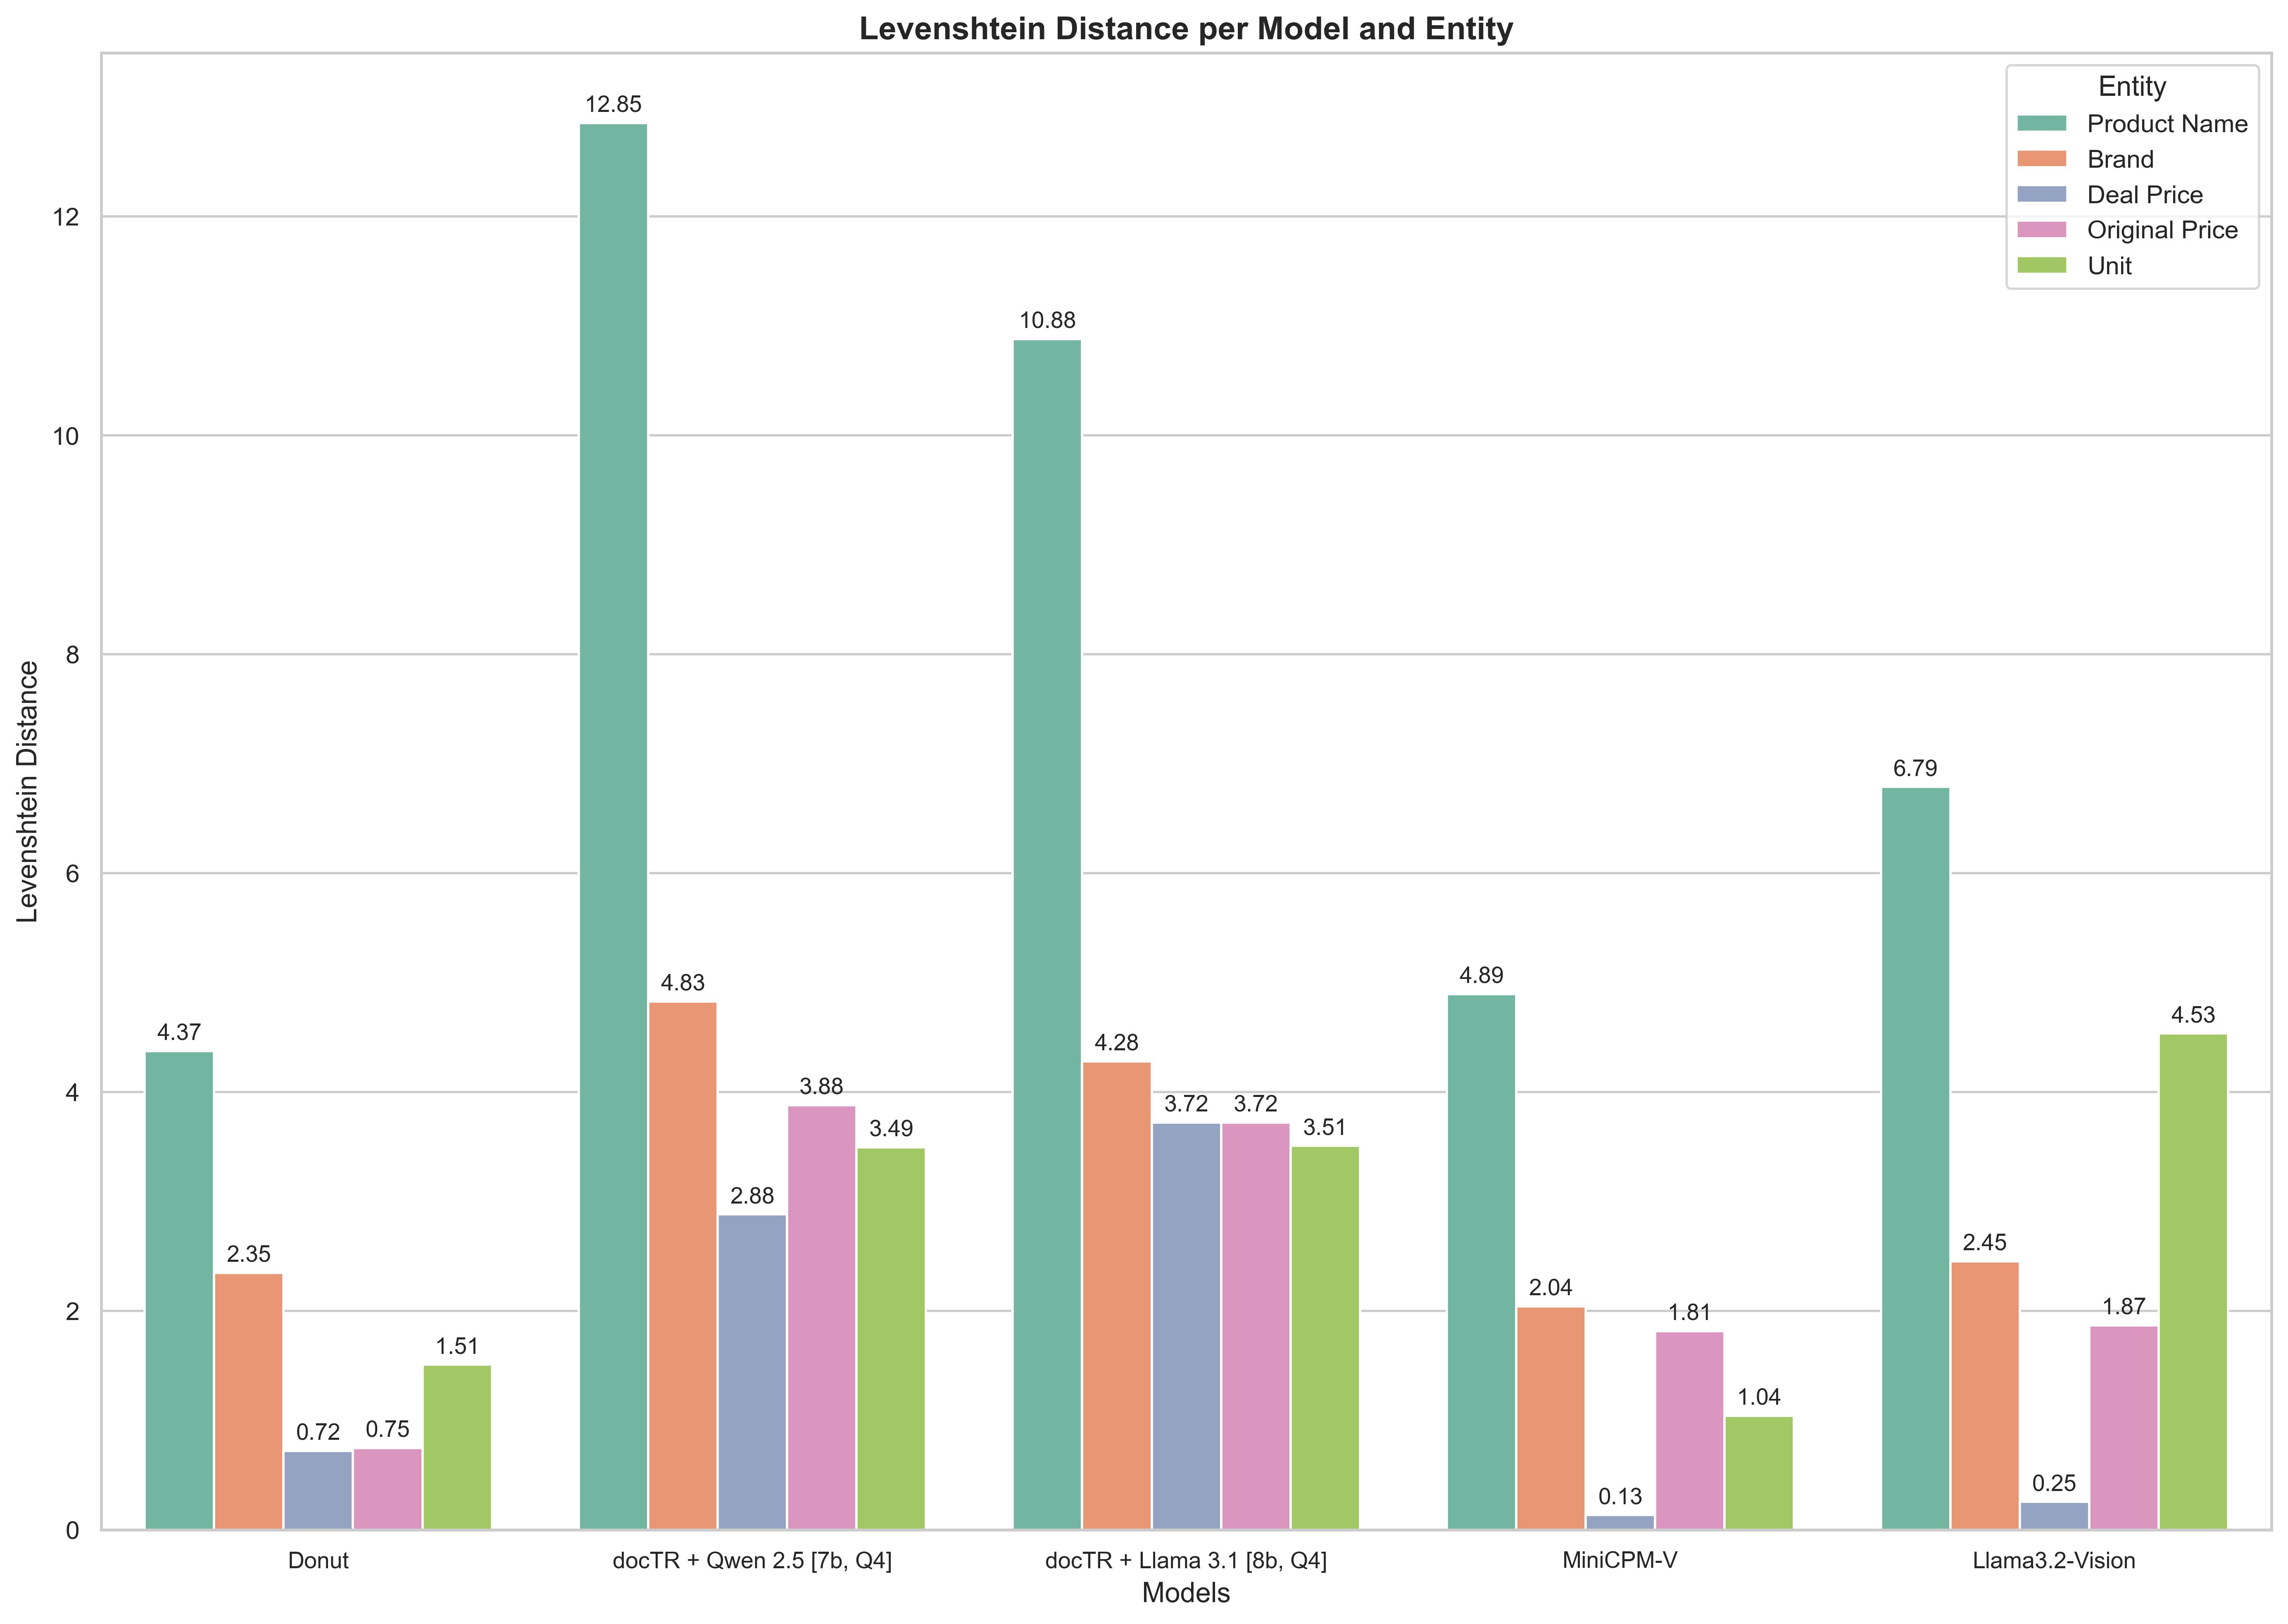
\includegraphics[width=0.8\linewidth]{figures/eval_final_levdis_raw.png}
    \caption{Per-Entity Levenshtein Distance without normalization.}
    \label{fig:eval_final_levdis_raw}
\end{figure*}

\begin{figure*}[h!]
    \centering
    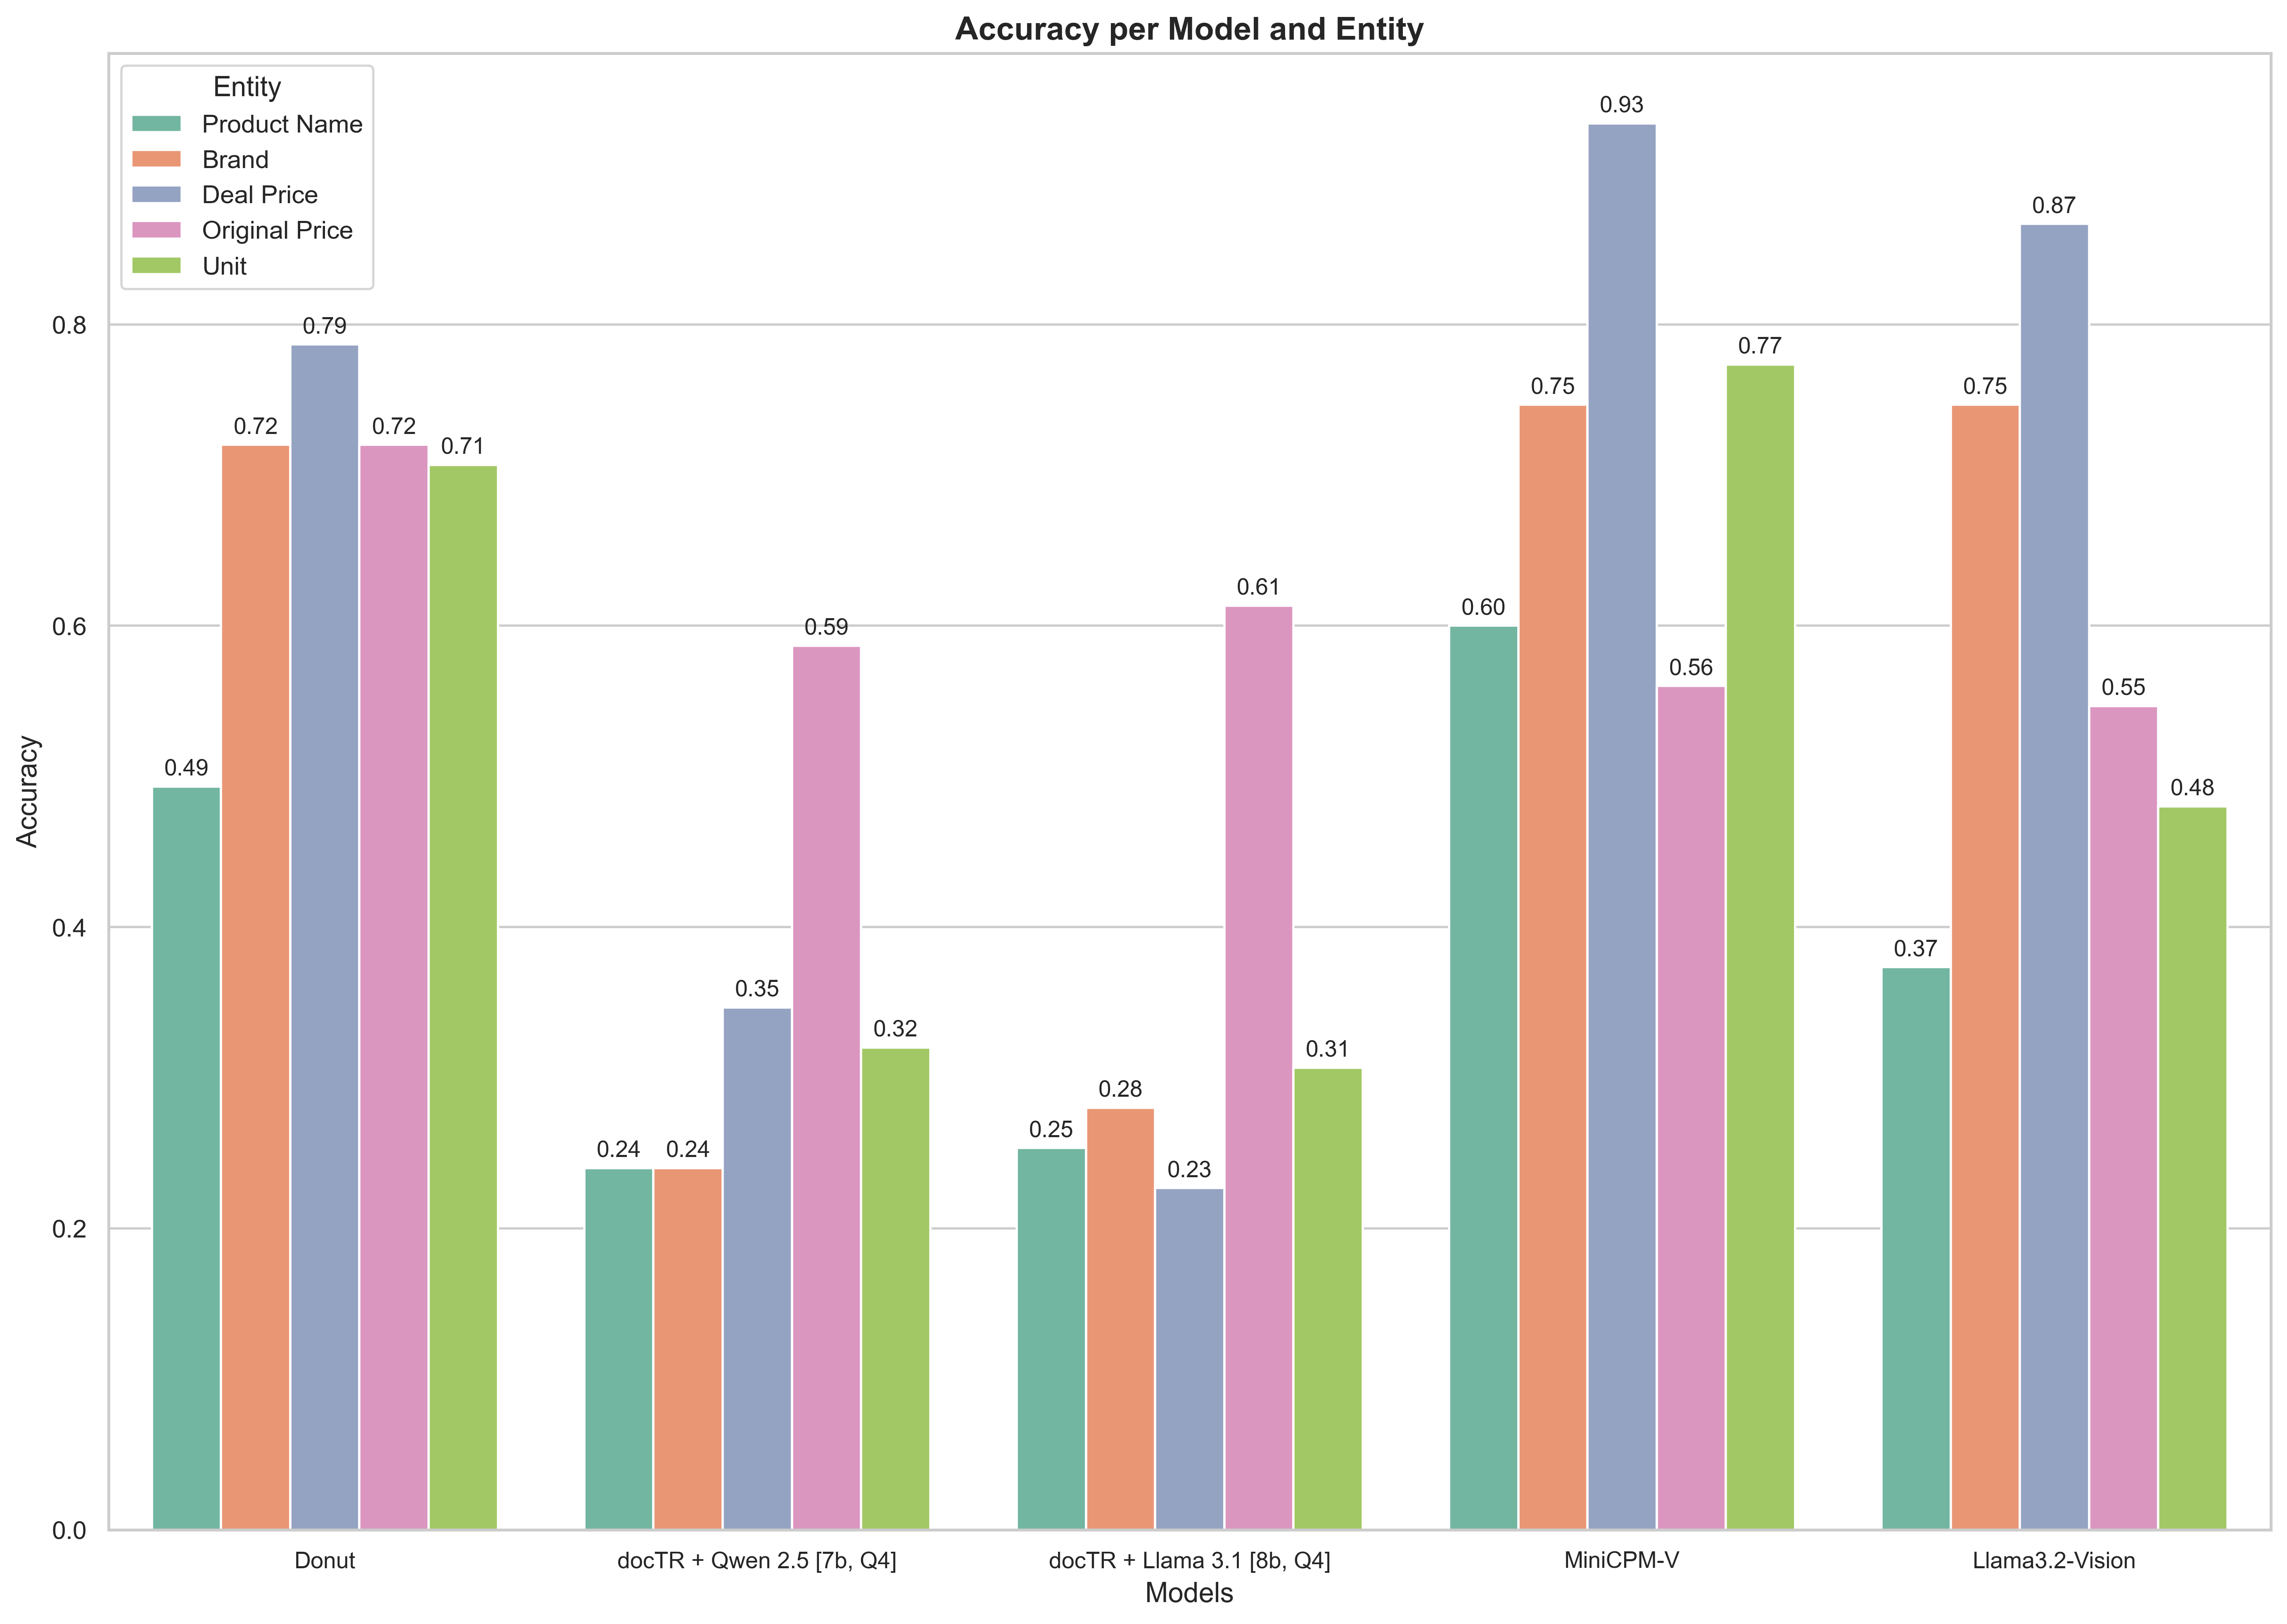
\includegraphics[width=0.8\linewidth]{figures/eval_final_acc_norm.png}
    \caption{Per-Entity Accuracy with normalization.}
    \label{fig:eval_final_acc_norm}
\end{figure*}

\begin{figure*}[h!]
    \centering
    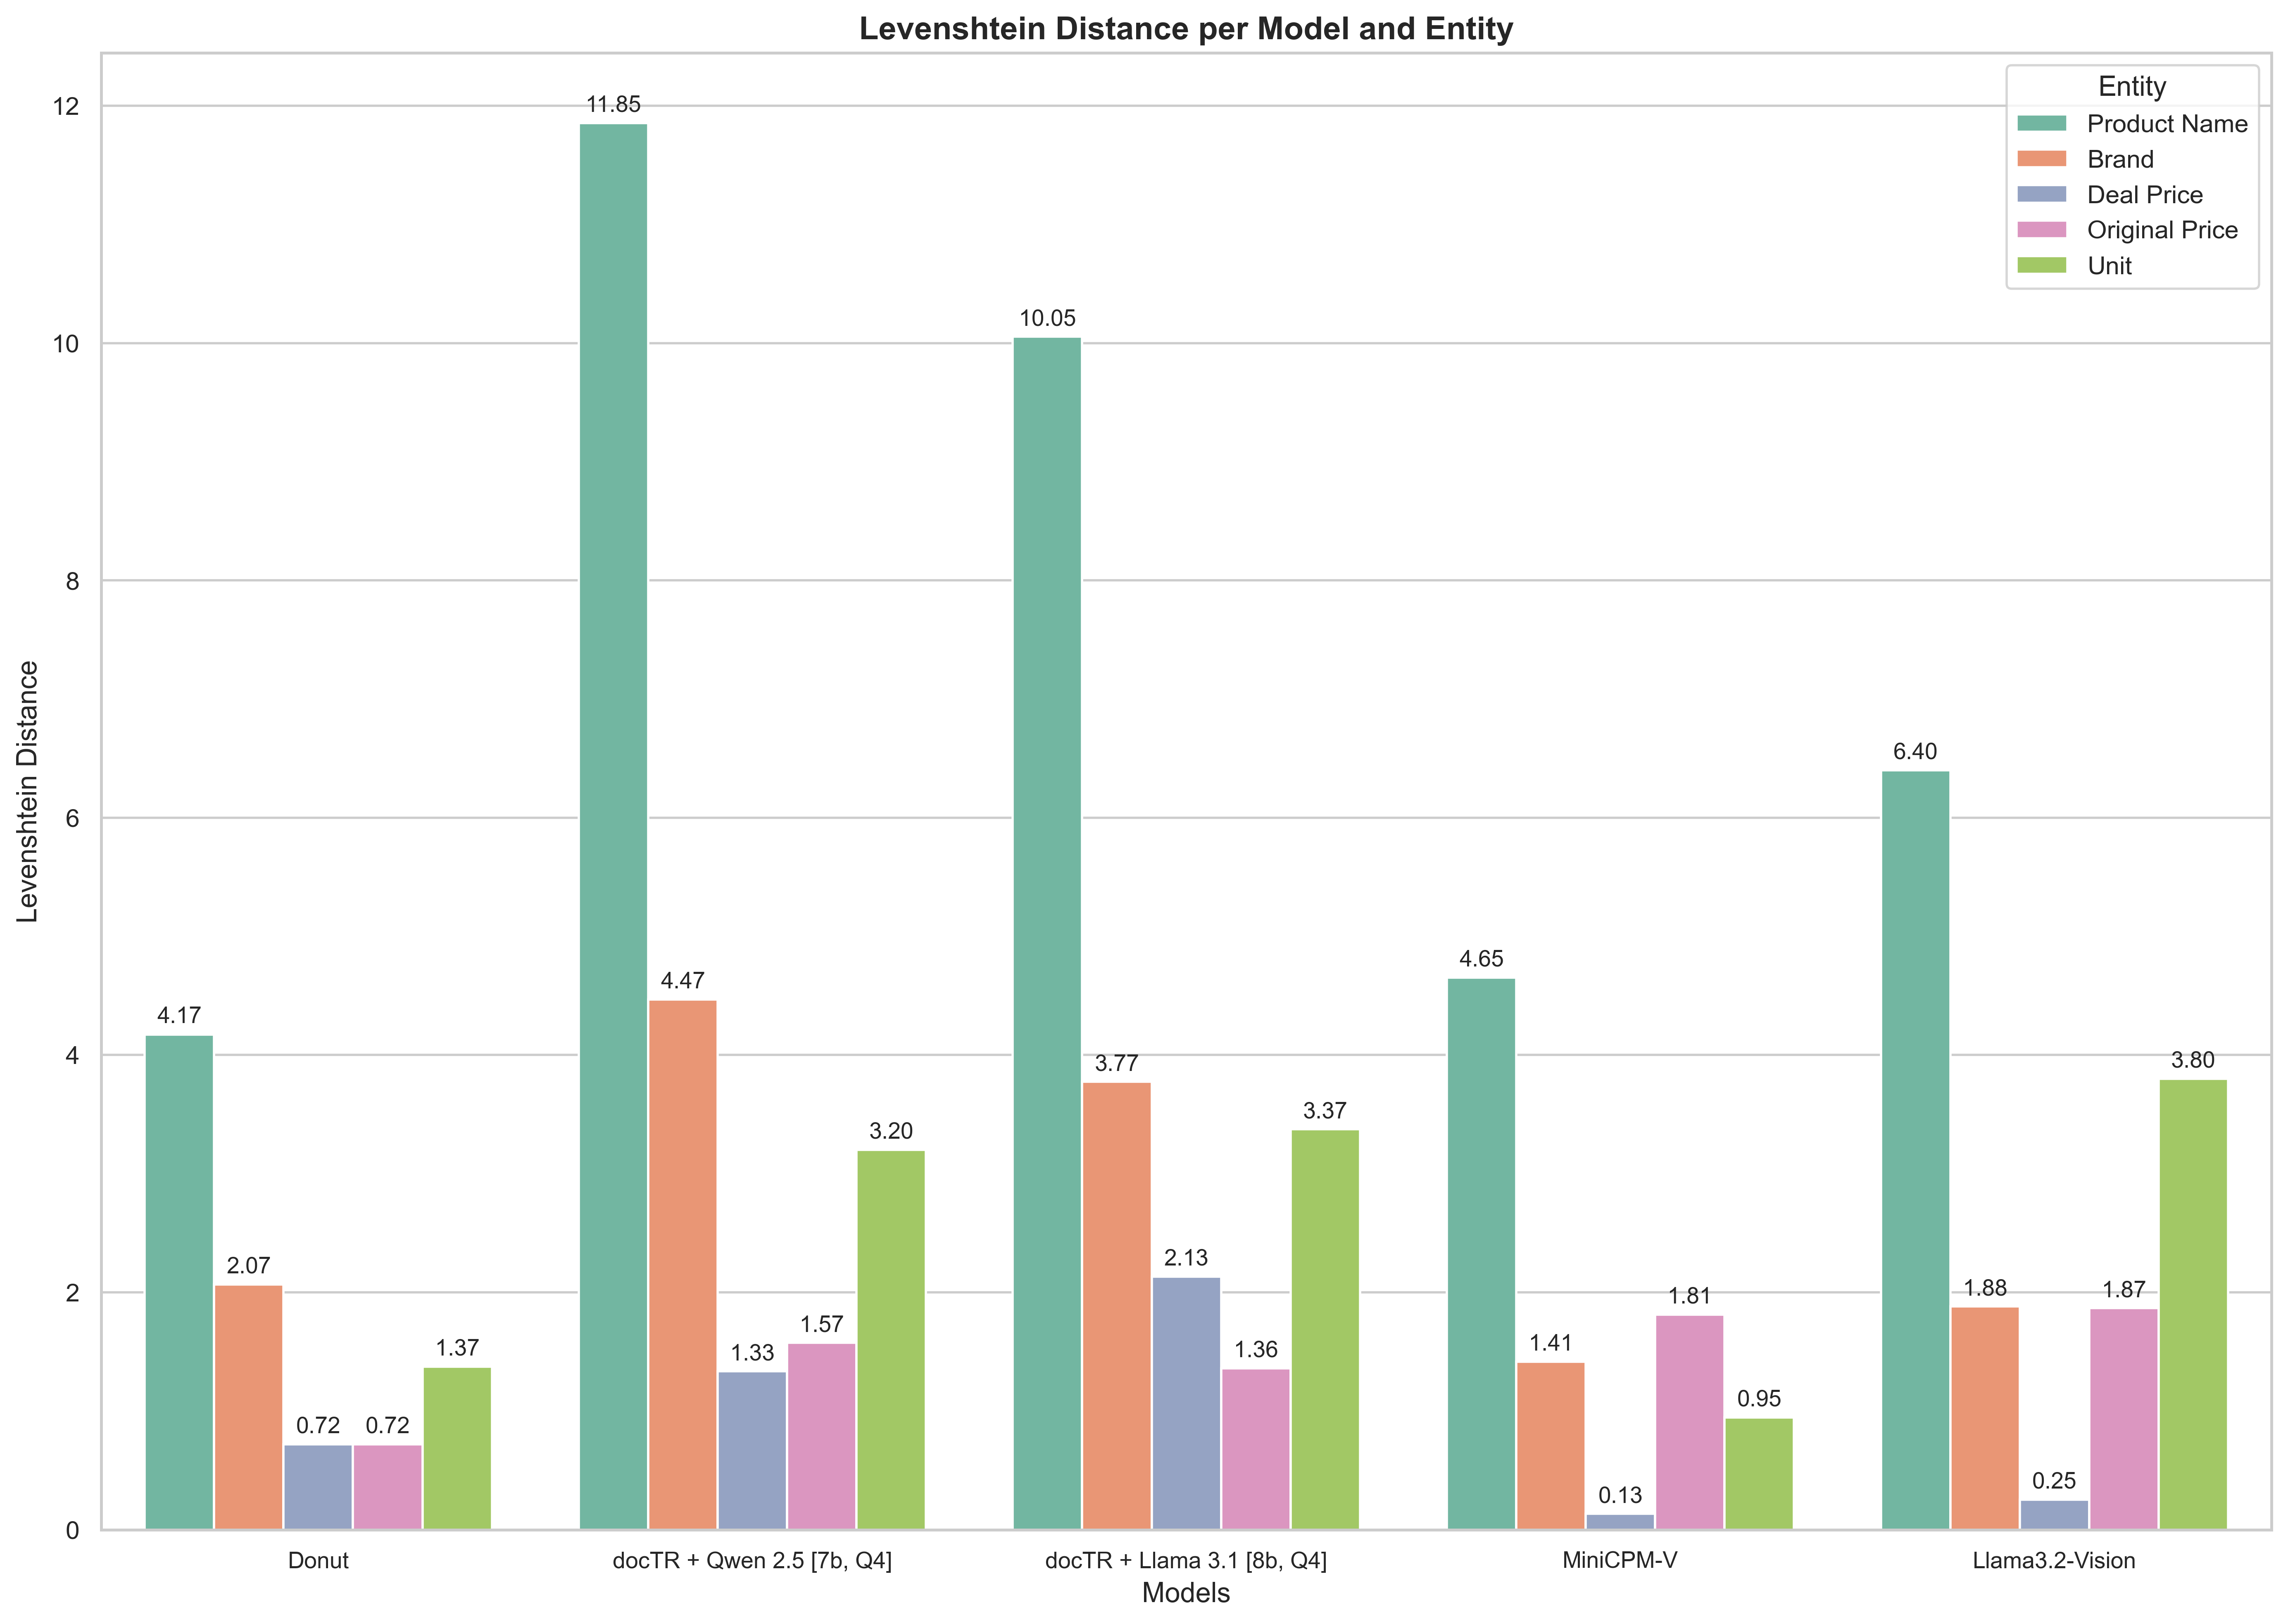
\includegraphics[width=0.8\linewidth]{figures/eval_final_levdis_norm.png}
    \caption{Per-Entity Levenshtein Distance with normalization.}
    \label{fig:eval_final_levdis_norm}
\end{figure*}





\section{Application}

\subsection{Database}



\section{Application}
    \section{Database}
    \section{Front End / Webapp}

\section{Conclusion}
    \subsection{Summary}
    \subsection{Future Work}
    ww




% Bibliography entries for the entire Anthology, followed by custom entries
%\bibliography{anthology,custom}
% Custom bibliography entries only
\bibliography{references}


\appendix
\section{Appendices}
\subsection{OCR Evaluation:Normalization Procedure}
% def normalize_text(text, level=6):
%     if not text or pd.isnull(text) or text == "":
%         return ""
    
%     # Level 1: Basic cleaning (handles empty values)
%     if level >= 1:
%         text = str(text).strip()
    
%     # Level 2: Lowercasing & basic replacements (whitespace, German characters)
%     if level >= 2:
%         text = text.lower()
%         text = text.replace("\n", " ").replace("\t", " ").replace("\r", " ")
%         text = text.replace("ö", "o").replace("ä", "a").replace("ü", "u").replace("ß", "ss")
    
%     # Level 3: Extended normalization (remove special characters, normalize hyphens)
%     if level >= 3:
%         text = text.replace("-", " ").replace("–", " ").replace("—", " ").replace("−", " ")
%         text = "".join([char for char in text if char.isalnum() or char in {".", " "}])
%         text = " ".join(text.split())  # Remove extra spaces

%     if level >= 4:
%         text = text.replace(" ", "")
%         text = text.replace(".", "")
%     return text

\subsection{LLM Prompt}
TODO

\subsection{OCR + LLM Evaluation: Normalization Procedure}

% \textbf{Normalization Procedure:}

% \begin{lstlisting}[language=Python, caption=Text Normalization Procedure]
% REPLACEMENTS = {
%     "ä": "a", "ö": "o", "ü": "u", "ß": "ss", ",": ".", "€": "",
%     "–": " ", "—": " ", "−": " ", "ô": "o", "é": "e", "ç": "c",
%     "è": "e", "à": "a", "ê": "e", "â": "a", "û": "u", "î": "i",
%     "ë": "e", "ï": "i", "œ": "oe", "æ": "ae", "ù": "u"
% }
% def normalize(text):
%     for key, value in REPLACEMENTS.items():
%         text = text.replace(key, value)
%     text = "".join([char for char in text if char.isalnum() or char in {".", " "}])
%     text = "".join(text.split())
%     return text.strip().lower()
% \end{lstlisting}
% TODO -> In appendix
% TODO: Continue

\end{document}
